\documentclass[12pt,twoside]{report}
\usepackage[margin=2.5cm]{geometry}
\linespread{1.375}
\usepackage[utf8]{inputenc}
\usepackage[T1]{fontenc}
\usepackage{polski}
\usepackage{listings}
\usepackage{indentfirst}
\usepackage[shortlabels]{enumitem}
\usepackage{multirow}
\usepackage{makecell}
\usepackage{float}
\usepackage{xcolor}
\usepackage{graphicx}
\usepackage{rotating}
\usepackage{lmodern} %Czcionka
\usepackage{wrapfig} %Tekst wokół obrazu
\raggedbottom %zwalcza dziwne rozciąganie
\begin{document}
	\begin{titlepage}
		
		\begin{center}
			\begin{figure}[t]
				\centering
			%	
\includegraphics[width=4.5cm,height=4.5cm]{LogoUO.jpg}
			\end{figure}
		\end{center}
		
		\begin{center}
			{\LARGE  \bf \textsc{UNIWERSYTET OPOLSKI}}
		\end{center}
		\vspace{0.2cm}
		\begin{center}
			{\large \textsc{Wydział Matematyki, Fizyki i Informatyki}}
		\end{center}
		%\vspace{0.2cm}
		\begin{center}
			{\Large \textsc{Instytut Informatyki}}
		\end{center}
		\vspace{0.5cm}
		\begin{center}
			\large    \textsc{Praca iżynierska}
		\end{center}
		\vspace{0.4cm}
		\begin{center}
			\large \textbf{Natalia Szymczak}
		\end{center}
		
		\vspace{0.4cm}
		\begin{center}
			\Large     \textbf{Aplikacja bazodanowa dla klubów jeździeckich}
		\end{center}
		\vspace{0.1cm}
		
		\begin{center}
			\large     \textsc{}
		\end{center}
		\vspace{1.3cm}
		
		\begin{flushright}
			{\large Praca wykonana pod kierunkiem\bigskip
				
				{\bf }} 
			dr. Jacka Iwańskiego
		\end{flushright}
		\vspace{0.7cm}
		\begin{center}
			{\large OPOLE 2022}
		\end{center}
	\end{titlepage}

	\thispagestyle{empty}
	\mbox{}
	
	\begin{quote}{\small 
			\noindent
			
			\bigskip
			\noindent
			\textbf{Streszczenie:} 
			
			
			\noindent
			\newline
			\textbf{}
			\vspace{5pt}
			
			\noindent
			\newline
			\textbf{Abstract:} 
			\vspace{5pt}
			
			\vspace{5pt}
			\noindent
			\newline
			\textbf{Keywords:} 
			\vspace{5pt}
			\bigskip
			
			\noindent 
			\textbf{Klasyfikacja tematyczna wg  MSC 2020:}}
	\end{quote}

	\mbox{}
	
	\pagestyle{plain}
	\tableofcontents
	\thispagestyle{empty}
	
	
	\newpage
	\setcounter{page}{1}
	\newpage
\chapter{Wstęp}
\chapter{Przegląd istniejących rozwiązań}
\chapter{Technologie użyte w pracy}
\section{Microsoft Visual Studio 2022}
\textcolor{red} {Microsoft Visual Studio to środowisko IDE, za pomocą którego można edytować, debugować jak także kompilować kod. Po stworzeniu aplikacji można ja także opublikować w prost ze środowiska. Środowisko to zawiera wiele funkcji wzbogacających proces tworzenia takich jak narzędzia uzupełniania kodu (Intellisense). Dzięki temu środowisku możemy programować aplikacje na dowolną platformę oraz dowolne urządzenia. }
\section{Microsoft SQL Server 2019 Express}
\textcolor{red} {Microsoft SQL Server jest to system, wspomagający zarządzanie bazą danych stworzony oraz utrzymywany przez firmę Microsoft. MS SQL wykorzystuje język zapytań Transact-SQL, który jest rozwinięciem standardu języka zapytań ANSI/SQL.}

\section{Microsoft SQL Server Management Studio}

\section{Structured Query Language}
\textcolor{red} {SQL czyli Structured Query Language jest to język zapytań wykorzystywany w relacyjnych bazach danych. Umożliwia on tworzenie, modyfikowania oraz zarządzanie bazami danych. Dodatkowo dzięki SQL jesteśmy w stanie pobierać, dodawać, aktualizować oraz usuwać dane znajdujące się w naszej bazie danych. SQL wspiera również tworzenie skomplikowanych zapytań, dzięki czemu możemy wykonywać różne operacje na danych takie jak: filtrowanie, sortowanie, grupowanie oraz łączenie.}

\section{Windows Presentation Foundation}
WPF - Windows Presentation Foundation, jest technologią opracowaną przez Microsoft. Służy ona do tworzenia aplikacji desktopowych na system Windows. Jest częścią .NET Framework i zapewnia on możliwość tworzenia zaawansowanych interfejsów użytkownika wykorzystując język XAML. Interfejs ten jest niezależny od rozdzielczości oraz używa aparatu renderowania opartego na wektorach, aby korzystać z nowoczesnego sprzętu graficznego. WPF dostarcza kontrolki, powiązanie danych, układ, grafike 2D i 3D, animację, style, szablony, dokumenty, multimedia, tekst i typografię, jak także inne elementy interfejsu API platformy .NET. \cite{WPF}

\section{Xamarin}
Xamarin jest to platforma do tworzenia aplikacji mobilnych za pomocą platformy .NET, która automatycznie obsługuje odzyskiwanie i alokowanie pamięci, jak także współdziałanie z platformami bazowymi. Dzięki Xamarinowi możemy pisać aplikacje na androida, iOS jak także na windows phone. Tworzy on warstwę abstrakcji komunikującą się za pomiędzy kodem aplikacji, a kodem bazowej platformy. Aplikacje wykorzystujące Xamarin możemy pisać nie tylko na komputerach PC z systemem Windows lub Linux, lecz także na urządzeniach z systemem MacOS. Architektura systemu Xamarin przedstawiona zostala na rysunku \ref{XamarinArchitecture}. Możemy na nim zobaczyć część architektury dotyczącą platformy android jak także, część dotyczącą platformy iOS.\cite{XamarinLearn}
\begin{figure}[H]
	\centering
	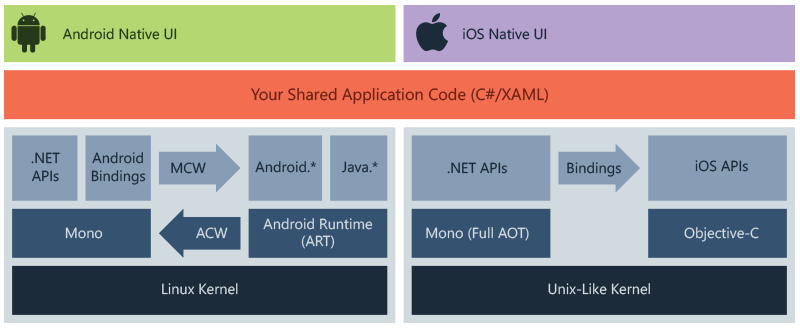
\includegraphics[scale=0.5]{xamarinArchitecture}
	\caption{Architektura platformy Xamarin}
	\textit{Źródło: \cite{XamarinLearn}}
	\label{XamarinArchitecture}
\end{figure}
\subsection{Xamarin.Android}
Aplikacja HorseTracking dostępna będzie jedynie na platformę android. Aby dostosować ją do systemu iOS niezbędne było by urządzenie z systemem MacOS co nie było możliwe.
Xamarin.Android kompilowany jest z języka C\#, do języka pośredniego "just in time", często nazywanego JIT od pierwszych liter nazwy. JIT jest skompilowany do zestawu natywnego po uruchomieniu aplikacji. Xamarin.Android jest uruchamiany w środowisku mono obok maszyny wirtualnej środowiska Android Runtime. Dzięki platformie Xamarin możemy powiązać platformę .Net z przestrzeniami nazw Android.* i Java.*. Za pośrednictwem zarządzanych otok wywoływanych MCW środowisko mono może wywoływać przestrzenie nazw oraz udostępniać otoki wywoływane przez system Android(ACW). Dzięki temu oba środowiska mogą wywoływać kod nawzajem. Na rysunku \ref{AndroidArchitecture} przedstawiona została architektura systemu Xamarin.Android\cite{XamarinLearn}.
\begin{figure}[H]
	\centering
	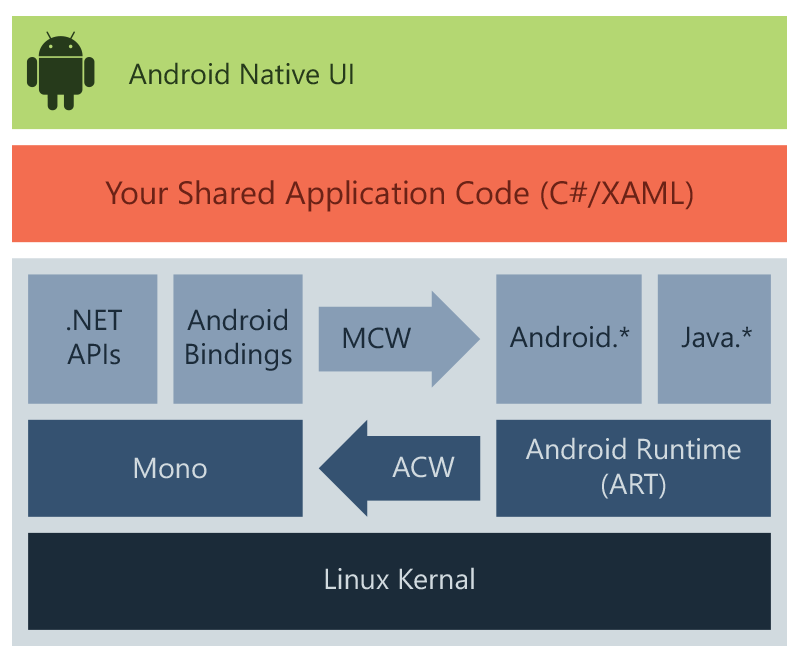
\includegraphics[scale=0.3]{androidArchitecture}
	\caption{Architektura platformy Xamarin.Android}
	\textit{Źródło: \cite{XamarinLearn}}
	\label{AndroidArchitecture}
\end{figure}

\section{Android Device Menager}

\section{NuGet}
NuGet (logo systemu na rysunku \ref{nugetLogo})jest to mechanizm udostępniania kodu obsługiwany przez firmę Microsoft. 
\begin{figure}[H]
	\centering
	
\includegraphics[scale=0.25]{nugetLogo}
	\caption{Logo systemu NuGet}
	\textit{Źródło: \cite{Nuget}}
	\label{nugetLogo}
\end{figure}
Służy on do współdzielenia kodu. Pakiet NuGet obsługuje hosty prywatne oraz publicznego hosta. Na hoście publicznym NuGet ma tysiące unikatowych pakietów dostępnych dla użytkowników .Net. Niezależnie od tego czy host jest prywatny czy publiczny jest on połączeniem między twórcami pakietów a ich konsumentami. Przepływ informacji między deweloperami pakietów, a ich konsumerami możemy zaobserwować na rysunku \ref{NugetFlow}.
\begin{figure}[H]
	\centering
	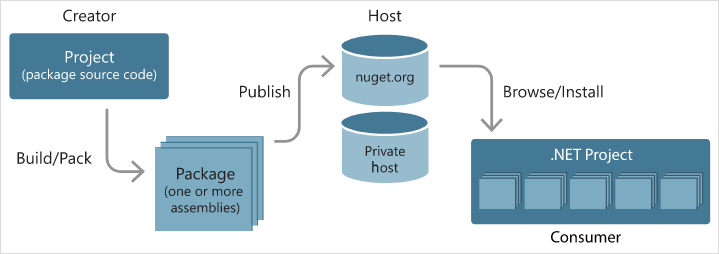
\includegraphics[scale=0.75]{nugetFlow}
	\caption{Przepływ informacji}
	\textit{Źródło: \cite{Nuget}}
	\label{NugetFlow}
\end{figure}
\section{Git}
Git, github, sourcetree

\section{Figma}
Figma jest to narzędzie do projektowania i prototypowania interfejsów aplikacji. Dzięki narzędziom takim jak figma możemy zaplanować cały interfejs jeszcze przed jego implementacją.  Stworzony w ten sposób interfejs możemy przetestować dzięki funkcji prototypowania. Jeszcze przed implementacją może on zostać udostępniony kilku osobą w celu sprawdzenia czy wszystkie funkcje aplikacji są dla użytkownika jasne i intuicyjne. Dzięki temu implementować będziemy interfejs już sprawdzony, więc będzie wymagał on mniej poprawek.
\begin{figure}[H]
	\centering
	\includegraphics[scale=0.15]{FigmaLogo}
	\caption{przepływ informacji}
	\textit{Źródło: \cite{FigmaIcon}}
	\label{FigmaLogo}
\end{figure}
\section{Entity Framework}
Entity Framework to narzędzie do mapowania obiektowo-relacyjnego, który umożliwia tworzenie przejrzystej, przenośnej i wysokopoziomowej warstwy dostępu do danych za pomocą platformy .NET (C\#) dla wielu baz danych.  Pozwala on na wykonywanie podstawowych operacji takich jak dodawanie, pobieranie, uaktualnianie i usuwanie danych. Możemy dzięki niemu także łatwiej zarządzać relacjami w bazie. Zasada działania tego narzędzia przedstawiona została na rysunku \ref{EntityArchitecture}
\begin{figure}[H]
	\centering
	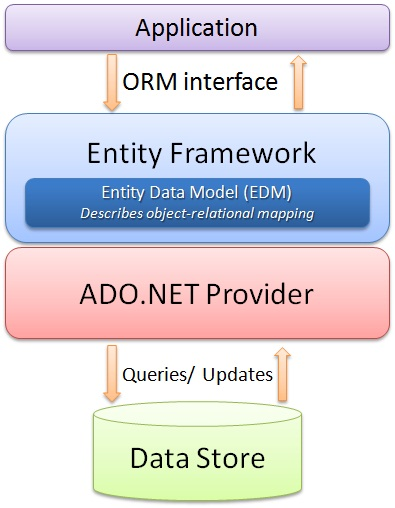
\includegraphics[scale=0.5]{EntityArchitecture}
	\caption{przepływ informacji}
	\textit{Źródło: \cite{Entity}}
	\label{EntityArchitecture}
\end{figure}
\section{Ten do wykresów}

\section{MVVM Toolkit}

\section{Xamarin Community Toolkit}

\section{ZXing.Net.Mobile.Forms}

\section{Microsoft.Extensions.DependencyInjection}
\chapter{Specyfikacja wymagań}
\section{Opis wycinka rzeczywistości}
Aplikacja przeznaczona jest dla klubów jeździeckich, czyli organizacji zrzeszających jeźdźców startujących w danej dziedzinie sportów konnych. Aplikacja skierowana jest do klubów, których zawodnicy startują w takich dziedzinach jak:
\begin{itemize}
	\item Skoki przez przeszkody,
	\item WKKW (skrót od "Wszechstronny konkurs konia wierzchowego"),
	\item Ujeżdżenie.
\end{itemize}

W celu jak najlepszego określenia wymagań funkcjonalnych, przed napisaniem aplikacji przeprowadzono rozmowy z kilkoma osobami zaangażowanymi w to środowisko: pracownikami stadnin państwowych, właścicielami klubów, jak także z osobami prywatnie trzymającymi konie w stadninach. Po przeprowadzonych rozmowach zdecydowano się na dwie wersje aplikacji: desktopową oraz mobilną, które będą różnić się funkcjonalnościami.

Aplikacja ma na celu pomóc w gromadzeniu informacji o jeźdźcach przynależących do klubu oraz ich koniach. W aplikacji gromadzone są informacje o codziennych aktywnościach koni, ich chorobach, żywieniu oraz zawodach w których biorą udział. Naturalnie chcemy także zapisywać wyniki z tych zawodów, aby móc określić czy dany trening jest skuteczny. Z aplikacji będą korzystać zawodnicy, trenerzy, jaki i zarząd klubu.

Aby skutecznie zbierać informacje o treningach i innych aktywnościach niezbędna jest aplikacja mobilna, ponieważ dane te muszą być wprowadzane na bieżąco. Informacje o wizytach różnorakich lekarz oraz kowala także muszą być zapisywane na bieżąco podczas danej wizyty. Dlatego funkcjonalności te dotyczą jedynie aplikacji mobilnej. W aplikacji mobilnej można również sprawdzić aktualny plan żywienia swojego konia. Do tej aplikacji będą mieć dostęp jedynie osoby posiadające konie. 

W aplikacji desktopowej wyświetlane są statystyki aktywności koni danego użytkownika jak i szczegóły wizyt lekarzy i kowali. W tej aplikacji można zaplanować wyjazdy na zawody jak także szczegółowe plany żywienia swoich podopiecznych. W tej aplikacji tworzone  będą także konta użytkowników, oraz ich koni. Dostęp do funkcji tworzenia kont będzie ograniczony i posiadać go będzie jedynie administrator aplikacji.

Każdy członek klubu będzie miał swoje konto z możliwością logowania zarówno do aplikacji mobilnej jak i desktopowej. Trenerzy, właściciele klubu i inne osoby związane z klubem będą miały dostęp jedynie do aplikacji desktopowej. 


\section{Wymagania funkcjonalne}
Funkcjonalności aplikacji mobilnej oraz desktopowej nie są takie same mimo iż są podłączone do jednej bazy, więc czerpią z tego samego źródła informacji. Pomimo znaczących różnic niektóre funkcjonalności pokrywają się w obu tych produktach. 
Wymagania funkcjonalne, które muszą spełniać obie aplikacje przedstawia tabelka \ref{funkcjonalneObuApek}.
%\renewcommand{\arraystretch}{1.5}
\begin{table}[H]
	\centering
\begin{tabular}{|p{4.5cm}|p{4cm}|p{7cm}|}			
	\hline
	Wymaganie & Aktor & Opis wymagania\\
	\hline
	Logowanie do aplikacji& Trener, Członek klubu, Zarząd klubu & System pozwala na zalogowanie się po podaniu poprawnego loginu oraz hasła.\\
	\hline
	Resetowanie hasła przez email & Trener, Członek klubu, Zarząd klubu& System umożliwia resetowanie hasła przez adres e-mail. \\
	\hline
	
\end{tabular}
	\caption{Wymagania funkcjonalne obu aplikacji}
	\label{funkcjonalneObuApek}
\end{table}

Aplikacja mobilna będzie służyć użytkownikom głównie do zapisu aktualnych wydarzeń z życia stajni. Jej głównym celem jest szybkie zapisanie informacji o aktywnościach koni i ich wizytach u lekarzy, bądź kowali. Można w niej także szybko sprawdzić przygotowany plan żywienia, oraz daty zbliżających się zawodów.
Wymagania funkcjonalne dla aplikacji mobilnej zawierają poniższe tabele \ref{funkcjonalneMobilki1} i \ref{funkcjonalneMobilki2}.
%\renewcommand{\arraystretch}{1.8}
\begin{table}[H]
	\centering
	\begin{tabular}{|p{3cm}|p{3cm}|p{3cm}|p{6cm}|}			
		\hline
	   \multicolumn{2}{|l|}{Wymaganie} & Aktor & Opis wymagania\\
		\hline
		Zarządzanie aktywnościami & Dodawanie aktywności & Członek klubu &  System umożliwia zapis danych wprowadzonych przez zalogowanego użytkownika do bazy danych.\\	
		\hline	
		Zarządzanie aktywnościami & Edytowanie aktywności & Członek klubu & System umożliwia edytowanie dodanych wcześniej danych o aktywnościach. \\	
		\hline	
		Zarządzanie aktywnościami& Usuwanie aktywności & Członek klubu & System pozwala na usuwanie dodanych wcześniej aktywności. \\
		\hline
		Zarządzanie aktywnościami& Wyświetlanie aktywności & Trener, Członek klubu, Zarząd klubu& System umożliwia na przeglądanie wszystkich danych o aktywnościach danego konia zgromadzonych w bazie danych.\\
		\hline
		Zarządzanie wizytami & Dodawanie wizyt & Członek klubu& System pozwala na zapisanie danych z wizyty konia u lekarza/kowala do bazy danych.\\
		\hline
		Zarządzanie wizytami & Edytowanie wizyt & Członek klubu& System powinien umożliwić zapis zaktualizowanych danych o wizycie do bazy.\\
		\hline
		Zarządzanie wizytami & Usuwanie wizyt & Członek klubu & System powinien umożliwiać usuwanie danych o dodanych wcześniej wizytach.\\
		\hline 
		Zarządzanie wizytami & Wyświetlanie wizyt & Trener, Członek klubu, Zarząd klubu& System powinien umożliwić przeglądanie danych o wizytach zgromadzonych w bazie.\\
		\hline
		Zarządzanie wizytami & Planowanie wizyt & Członek klubu & System powinien pozawalać użytkownikom na dodanie do bazy danych o następnej wizycie, czyli umożliwić zapis wizyt jedynie z datą i opisem.\\
		\hline
		Zarządzanie wizytami & Zapisywanie zdjęcia z wizyty & Członek klubu&System powinien pozwalać na zapisywanie zdjęci z wizyt.\\
		\hline
	\end{tabular}
	\caption{Wymagania funkcjonalne aplikacji mobilnej}
	\label{funkcjonalneMobilki1}
\end{table}

%\renewcommand{\arraystretch}{1.8}
\begin{table}[h!]
	\centering
	\begin{tabular}{|p{3cm}|p{3cm}|p{4cm}|p{6cm}|}			
		\hline
		\multicolumn{2}{|l|}{Wymaganie} & Aktor & Opis wymagania\\
		\hline
		Zarządzanie wizytami & Przypomnienia o wizytach& Członek klubu & System powinien wysłać powiadomienie o zbliżającej się wizycie\\
		\hline
		Zarządzanie żywieniem & Przeglądanie planów żywienia & Członek klubu & System powinien umożliwiać przeglądanie planów żywienia umieszczonych w bazie.\\
		\hline
		Zarządzanie żywieniem & Wybór planu żywienia & Członek klubu & System powinien umożliwiać wybór jednego z planów żywienia umieszczonych w bazie jako tego aktualnie używanego.\\
		\hline
		Zarządzanie zawodami & Wyświetlanie najbliższych zawodów & Członek klubu & System powinien umożliwić wyświetlanie dat najbliższych zawodów umieszczonych w bazie.\\
		\hline
		Zarządzanie zawodami & Potwierdzenie udziału w zawodach & Członek klubu & System powinien umożliwić użytkownikowi potwierdzenie swojego udziału w zawodach.\\
		\hline
		\multicolumn{2}{|l|}{Udostępnianie koni}&Członek klubu& System powinien umożliwić udostępnianie koni między użytkownikami.\\
		\hline
	\end{tabular}
	\caption{Wymagania funkcjonalne aplikacji mobilnej}
	\label{funkcjonalneMobilki2}
\end{table}

Aplikacja desktop-owa przeznaczona jest zarówno dla użytkowników posiadających swoje konie jak i dla osób zarządzających klubem jeździeckim. W aplikacji desktop-owej posiadacze koni będą mogli obejrzeć zgromadzone informacje w przystępniejszej formie na dużym ekranie, stworzyć plan żywienia swojego konia, jak także przeanalizować statystki swoich koni. Osoby zarządzające klubem będą miały możliwość dodawania nowych użytkowników i koni jak także sprawdzania statystyk wszystkich koni klubowych. Szczególowe wymagania funkcjonalne dla aplikacji desktopowej zostały przedstawione w tabelach \ref{funkcjonalneDesktop1} oraz \ref{funkcjonalneDesktop2}.
%\renewcommand{\arraystretch}{1.8}
\begin{table}[H]
	\centering
	\begin{tabular}{|p{3cm}|p{3cm}|p{4cm}|p{6cm}|}			
		\hline
		\multicolumn{2}{|l|}{Wymaganie} & Aktor & Opis wymagania\\
		\hline
		Zarządzanie planami żywienia & Tworzenie planów żywienia  & Członek klubu & System umożliwia użytkownikowi stworzenie planu żywienia i zapisanie go do bazy.\\		
		\hline
		Zarządzanie planami żywienia & Edytowanie planów żywienia  & Członek klubu & System pozwala aktualizować stworzone wcześniej plany żywienia.\\
		\hline
		Zarządzanie planami żywienia & Usuwanie planów żywienia  & Członek klubu & System umożliwia usuwanie danych o stworzonych wcześniej planach żywienia.\\
		\hline
		Zarządzanie końmi& Dodawanie koni & Zarząd klubu & System umożliwia wprowadzenie danych o koniach i dodanie ich do konkretnego użytkownika\\ 		
		\hline
		Zarządzanie końmi& Usuwanie koni & Zarząd klubu & System umożliwia usuwanie koni\\ 		
		\hline
		Zarządzanie końmi& Edytowanie koni & Zarząd klubu & System umożliwia edycję danych o koniach zgromadzonych już w bazie.\\ 
		\hline
		Zarządzanie użytkownikami & Dodawanie użytkowników & Zarząd klubu & System umożliwia dodawanie danych o użytkownikach i tworzenie ich kont.\\		
		\hline
		Zarządzanie użytkownikami & Edytowanie użytkowników & Zarząd klubu & System umożliwia edytowanie danych użytkownika\\		
		\hline
		Zarządzanie użytkownikami & Usuwanie użytkowników & Zarząd klubu & System umożliwia usuwanie użytkowników\\
		\hline
		Zarządzanie użytkownikami & Zmiana hasła & Zarząd klubu,Członek klubu, Trener& System umożliwia zmianę hasła przez użytkownika.\\
		\hline
		
	\end{tabular}
\caption{Wymagania funkcjonalne aplikacji desktopowej}
\label{funkcjonalneDesktop1}
\end{table}
%\renewcommand{\arraystretch}{1.8}
\begin{table}[h!]
	\centering
	\begin{tabular}{|p{3cm}|p{3cm}|p{4cm}|p{6cm}|}			
		\hline
		\multicolumn{2}{|l|}{Wymaganie} & Aktor & Opis wymagania\\
		\hline
		Zarządzanie zawodami & Dodawanie zawodów & Zarząd klubu& System pozwala na tworzenie zawodów, oraz zapraszanie do udziału w nich poszczególnych członków klubu\\	
		\hline	
		Zarządzanie zawodami & Edytowanie zawodów & Zarząd klubu& System pozwala na edycję danych o dodanych wcześniej zawodach\\
		\hline
		Zarządzanie zawodami & Usuwanie zawodów & Zarząd klubu& System pozwala na usuwanie danych o dodanych wcześniej zawodach.\\
		\hline
		\multicolumn{2}{|l|}{Przeglądanie histori wizyt}& Członek klubu, Trener, Zarząd klubu&\\
		\hline
		\multicolumn{2}{|l|}{Przeglądanie statystyk}&Członek klubu, Trener, Zarząd klubu&\\
		\hline
	\end{tabular}
	\caption{Wymagania funkcjonalne aplikacji desktopowej}
	\label{funkcjonalneDesktop2}
\end{table}
\newpage
$\ $
\newpage
\subsubsection{Przypadki użycia}
Wszystkie wymagania funkcjonalne zgromadzone w powyższych tabelach, możemy przedstawić na diagramie przypadków użycia UML. Poniższe rysunki zostały sporządzone według zasad języka UML, opisanych w pozycji[odnieść się do bibliografi]. Na rysunku \ref{UseCaseDesktop} przedstawione zostały przypadki użycia aplikacji desktopowej, zaś na rysunku \ref{UseCaseMobile} przedstawione zostały przypadki użycia aplikacji mobilnej.
\begin{figure}[H]
	\centering
	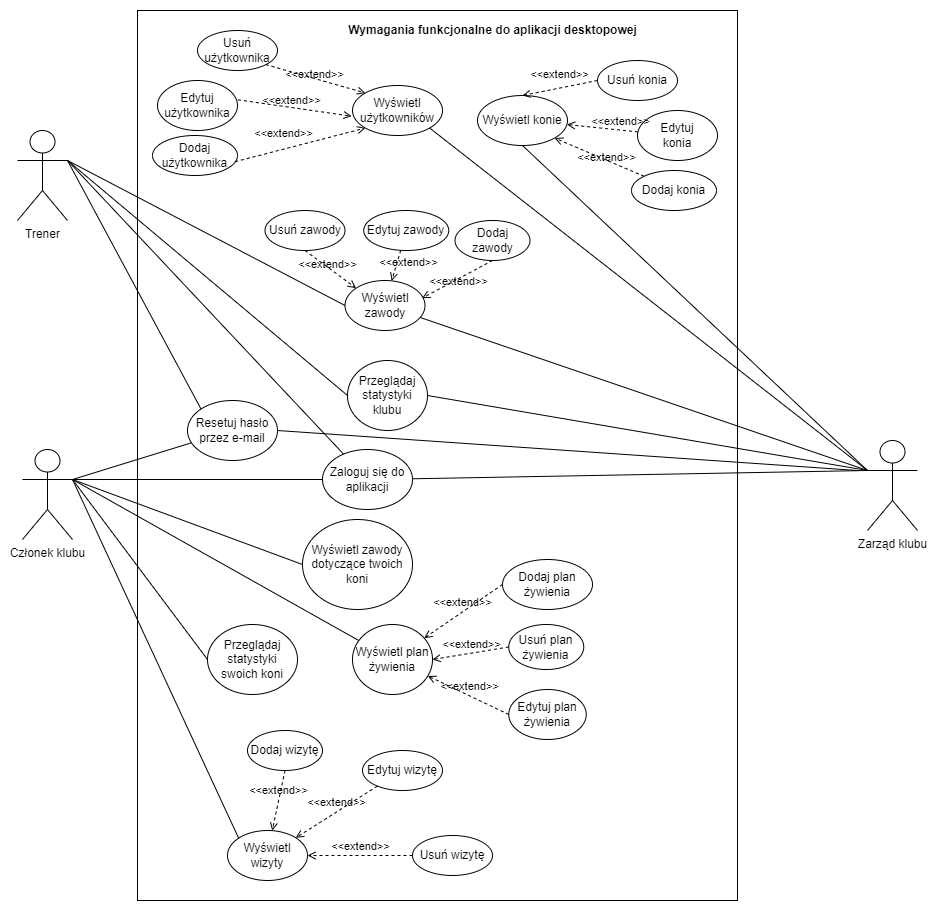
\includegraphics[scale=0.5]{UseCaseDesktop}
	\caption{Diagram Use Case dla aplikacji desktopowej}
	\textit{Źródło: Opracowanie własne}
	\label{UseCaseDesktop}
\end{figure}

\begin{figure}[H]
	\centering
	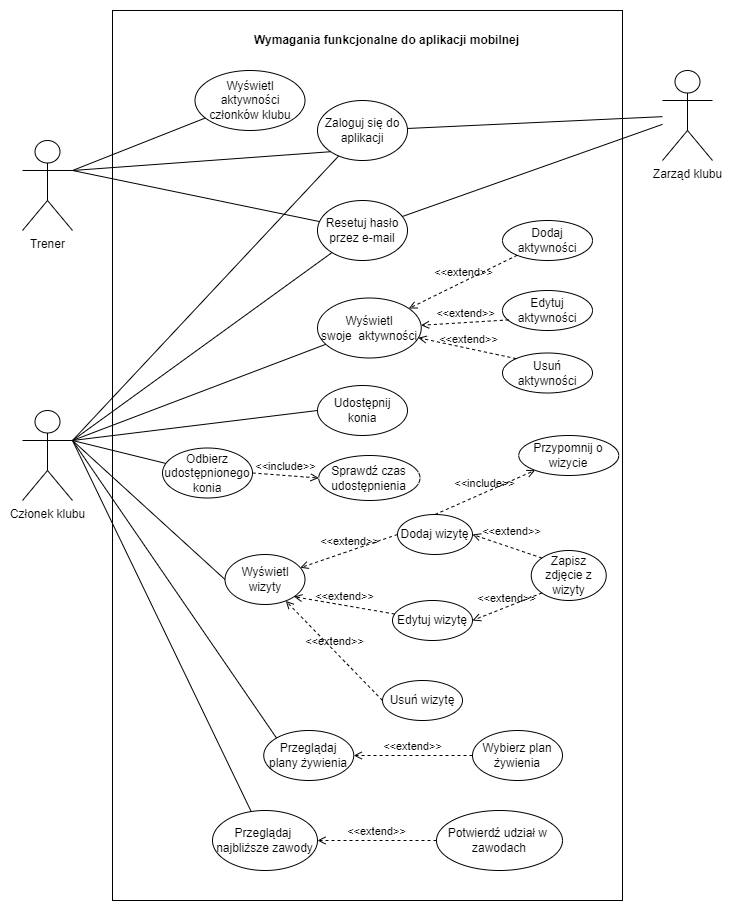
\includegraphics[scale=0.6]{UseCaseMobile}
	\caption{Diagram Use Case dla aplikacji mobilnej}
	\textit{Źródło: Opracowanie własne}
	\label{UseCaseMobile}
\end{figure}
\newpage
\section{Wymagania niefunkcjonalne}
W tym rozdziale przedstawione zostana wymagania niefunkcjonalne projektowanego systemu. W osobnych tabelach przedstawione zostaną wymagania dla aplikacji mobilnej (tabela \ref{}) oraz desktopowej (tabela \ref{WymaganiaNFdesktop}). 
Przedstawione wymagania zostały opracowane zgodnie ze standardem ISO 9126. Określone zostały atrybuty, takie jak: niezawodność (Reliability), obsługiwalność(Usability), wydajność(Efficiency), łatwość konserwacji (Maintainability) i przenośność(Portability).
	\begin{table}[H]
	\caption{Wymagania niefunkcjonalne aplikacji desktopowej }
	\textit{Źródło: Opracowanie własne}
	\label{WymaganiaNFdesktop}
	\centering
	\begin{tabular}{|c|c|p{8cm}|}
		\hline
		Nr & Nazwa wymagania & Opis wymagania\\
		\hline
		1& Interfejsy programowe& System operacyjny Microsoft Windows 7 lub nowszy. Baza danych zainstalowana na platformie Microsoft SQL Server 2019 lub nowszej oraz dostępna dla aplikacji zgodnie z zasadami określonymi w dokumentacji serwera.\\		
		\hline
		2& Interfejsy sprzętowe& Komputer osobisty lub laptop, obsługujący system Windows 7 lub nowszy. Minimum 4 GB pamięci RAM i xGB wolnej przestrzeni na dysku, procesor 1GHz lub szybszy, 32 bitowy (x86) lub 64 bitowy (x64).\\	
		\hline	
		3& Obsługiwaloność (Usability)& Aplikacja powinna mieć prosty i intuicyjny interfejs użytkownika. Interfejs powinien być dostosowany do pracy na monitorach o małej rozdzielczości i laptopach.\\		
		\hline
		4& Niezawodność (Reliability)& Aplikacja powinna walidować wszystkie pola, do których wprowadzane są dane. W przypadku błędnych danych powinny wyświetlać się komunikaty informujące o nieprawidłowościach w klarowny sposób.\\	
		\hline
		5& Język i narzędzia programowania& Aplikacja została napisana w C\# na silniku graficznym Windows Presentation Foundation przy użyciu środowiska  Microsoft Visual Studio Community 2022.
		Baza danych została napisana w języku SQL, przy pomocy środowiska Microsoft SQL Server Management Studio 18 i zainstalowana na serwerze bazy danych Microsoft SQL Server 2019\\	
		\hline
	\end{tabular}
\end{table}
\begin{table}
\begin{tabular}{|c|c|p{8cm}|}
					\hline
		6& Aspekty prawne& W bazie danych przechowywane będą dane członków klubu, zarządu, specjalistów oraz których korzystają. Poza danymi osobowymi tych osób przechowywane będą także dane o koniach, ich aktywnościach oraz stanie zdrowia. Aplikacja nie będzie przekazywać danych ososobowych poszczególnych członków innym użytkownikom.Dane specjalistów będą rozpowszechniane między użytkownikami, dlatego przed wpisaniem do bazy będą musieli wyrazić na to pisemną zgodę.\\	
				\hline
		7& Wydajność (Efficiency)& Używanie aplikacji na sprzęcie o minimalnych wymaganiach powinno przebiegać w sposób płynny, to znaczy wyświetlanie, dodawanie, edytowanie, usuwanie, kategoryzowanie i filtrowanie danych powinno nie zajmować dłużej niż kilka sekund.\\	
		\hline
		8& Łatwość konserwacji (Maintainability)& Działanie aplikacji będzie kontrolowane przy pomocy dziennika debugowania. Kolejne wersje systemu (kopie zapasowe) będą zapisywane za pomocą systemu kontroli wersji GIT.\\	
		\hline
		9& Przenośność (Portability)& Aplikacja udostępniana będzie w pliku wykonywalnym .exe. Baza danych musi zostać zainstalowana i skonfigurowana na serwerze w danym klubie jeździeckim. Po zainstalowaniu aplikacja i baza danych powinny zostać skonfigurowane ze sobą.\\
		\hline
	\end{tabular}
\end{table}

\begin{table}[H]
	\caption{Wymagania niefunkcjonalne aplikacji mobilnej }
	\textit{Źródło: Opracowanie własne}
	\label{WymaganiaNFmobilne}
	\centering
	\begin{tabular}{|l|l|p{8cm}|}
		\hline
		Nr & Nazwa wymagania & Opis wymagania\\
		\hline
		1& Interfejsy programowe& Android ?? lub nowszy \\		
		\hline
		2& Interfejsy sprzętowe& Telefon lub tablet z systemem operacyjnym Android ?? lub nowszym \\	
		\hline	
		3& Obsługiwaloność (Usability)& 
		Aplikacja powinna dobrze skalować się na różnej wielkości ekrany. Na telefonie najważniejsze przyciski powinny znajdować się "w zasięgu kciuka". Ikony i przyciski powinny być widoczne i możliwe do kliknięcia nawet małych ekranach (minimalny ekran ??), w aplikacji dostępny jest jedynie tryb jasny.\\		
		\hline
		4& Niezawodność (Reliability)&Aplikacja powinna walidować wszystkie pola, do których wprowadzane są dane. W przypadku błędnych danych powinny wyświetlać się komunikaty informujące o nieprawidłowościach w klarowny sposób. \\	
		\hline
		5& Język i narzędzia programowania& Aplikacja została napisana na platformie Xamarin przy użyciu środowiska  Microsoft Visual Studio Community 2022. Używa tej samej bazy co aplikacja desktopowa. \\	
		\hline
		6& Aspekty prawne& Aspekty prawne aplikacji mobilnej i desktopowej pokrywają się, ponieważ korzystają one z tych samych danych.\\	
		\hline
		7& Wydajność (Efficiency)&
		Używanie aplikacji na sprzęcie o minimalnych wymaganiach powinno przebiegać w sposób płynny, to znaczy wyświetlanie, dodawanie, edytowanie, usuwanie danych powinno nie zajmować dłużej niż kilka sekund. \\	
		\hline
		8& Łatwość konserwacji (Maintainability)&
		Konserwacja aplikacji mobilnej będzie przebiegać analogicznie do desktopowej. \\	
		\hline
		9& Przenośność (Portability)&Aplikacja udostępniana w postaci pakietu instalacyjnego .apk oraz powinna spełniać wszystkie wymagania do umieszczenia jej w sklepie Google Play. \\
		\hline
		
	\end{tabular}
\end{table}

\newpage
\chapter{Baza danych}
W tym rozdziale przedstawimy model konceptualny, logiczny oraz fizyczny bazy danych. Rozdział ten został opracowany na podstawie \cite{bazydanych}.
\section{Model konceptualny}
Proces tworzenia bazy danych zaczynamy od modelu konceptualnego. W pierwszej fazie tworzenia go ważne jest określenie słownika pojęć, które będą następnie używane w projekcie bazy danych.
\subsubsection{Słownik pojęć}
\begin{itemize}
	\item \textbf{Użytkownik} - wszyscy członkowie klubu, trenerzy oraz zarząd klubu.
	\item \textbf{Koń} - koń należący do któregoś z członków klubu jeździeckiego, lub dzierżawiony przez niego.
	\item \textbf{Atywności} - są to czynności wykonywane przez konia w ciągu dnia, należą do nich jazdy, skoki przez przeszkody, kross, ujeżdżenie, lonża, wyjazd w teren, karuzela, padok, wyjazd na zawody, spacer, skoki luzem, padok.
	\item \textbf{Wizyty} - to wizyty wszelkich lekarzy, jak także wizyty kowali.
	\item \textbf{Udostępnianie konia} - jest to przekazanie możliwości wprowadzania danych o danym koniu przez jego właściciela innemu członkowi klubu.
	
\end{itemize}
\newpage
Po określeniu definicji poszczególnych pojęć używanych w projekcie możemy przystąpić do tworzenia kategorii.
\subsubsection{Kategorie}
Po przeanalizowaniu wycinku rzeczywistości możemy określić jakie dane chcemy zbierać i zapisywać do bazy danych. Dane te możemy podzielić na kategorie i opisać językiem naturalnym ich cechy charakterystyczne.
\begin{enumerate}[start=1,label={\bfseries KAT:\arabic*}]
	\item 
\end{enumerate}
\newpage
Po określeniu kategorii możemy określić reguły funkcjonowania naszej aplikacja.
\subsubsection{Reguły funkcjonowania}
Reguły funkcjonowania określają zasady, procedury i wytyczne jakie musi spełniać projektowana aplikacja. 
\begin{enumerate}[start=1,label={\bfseries REG\textbackslash 00\arabic*}]
	\item Konta użytkowników tworzy jedynie użytkownik "administrator".
	\item Każdy użytkownik ma określony swój typ.
	\item Każdy użytkownik może zmienić swoje hasło.
	\item O każdym użytkowniku, jak także o lekarzu i kowalu zbieramy podstawowe dane personalne.
	\item Tylko użytkownik "administrator" dodaje konie do kont użytkowników.
	\item Każdy koń ma przypisaną płeć.
	\item Każdy koń ma przypisany status.
	\item Jeden użytkownik może posiadać wiele koni.
	\item Aktywności konia może dodać jego właściciel lub osoba której właściciel udostępni konia.
\end{enumerate}
\begin{enumerate}[start=10,label={\bfseries REG\textbackslash 0\arabic*}]
	\item Koń może mieć wiele aktywności każdego dnia.
	\item Wizyty konia może dodawać tylko jego właściciel.
	\item Na wizycie jest jeden koń i jedne lekarz/kowal.
	\item Każdy lekarz ma określoną specjalizacje.
	\item Plan żywienia konia może ustalać tylko właściciel. 
	\item Koń może posiadać wiele planów żywienia, ale aktualnie może jeść tylko jeden.
	\item Plan żywienia zawiera wiele żywień.
	\item Żywienie dotyczy konkretnego typu jedzenia, podawanego o konkretnej porze (rano, południe, wieczór), który swoją jednostkę miary.
	\item Użytkownicy, którym ktoś udostępnił konia mogą tylko wyświetlić plan żywienia.
	\item Statystyki mają być tworzone na podstawie aktywności.
	\item Użytkownik "członek klubu" może przeglądać statystyki tylko swoich koni.
	\item Użytkownik "trener" lub "administrator" może przeglądać statystyki wszystkich koni.
	\item Użytkownik "trener" lub "administrator" może dodawać wyjazd na zawody dla całego klubu i zapraszać poszczególnych użytkowników.
	\item Użytkownik "członek klubu" może dodawać swoje wyjazdy na zawody.
\end{enumerate}
\newpage
\subsubsection{Ograniczenia dziedzinowe}
Ograniczenia dziedzinowe to ograniczenia, które nakładane są na atrybuty w powyższych kategoriach. Wynikają one z analizy wycinka rzeczywistości i należy je uwzględnić podczas projektowania bazy danych oraz implementacji systemu.
\begin{enumerate}[start=1,label={\bfseries OGR\textbackslash 00\arabic*}]
	\item Paszport konia składa się ze znaków i cyfr postaci xxx-aaa-bb-ccccc-dd, gdzie
	\begin{itemize} 
		\item xxx - określa kraj pochodzenia konia,  
		\item aaa - oznacza kod hodowli konia, 
		\item bb- oznacza rok urodzenia konia, 
		\item ccccc - to numer paszportu konia, 
		\item dd - to numer identyfikacyjny konia w ramach hodowli.
		\end{itemize}
	\item Data wizyty konia jest wcześniejsza niż data jego urodzenia.
	\item 
\end{enumerate}
\newpage
\subsubsection{Transakcje}
Transakcje są to operacje, które możemy wykonywać na danych. Mają one cztery własności, które w skrócie nazywamy ACID (ang. Atomicity, Consistency, Isolation, Durability). Transakcje mają więc następujące własności:
\begin{itemize}
	\item atomowość, inaczej niepodzielność oznacza, że transakcje muszą być wykonywane na bazie w całości. Jeśli transakcja nie zostanie poprawnie przeprowadzona należny przywrócić stan bazy z przed jej wykonania.
	\item spójność, po wykonaniu transakcji baza powinna być nadal spójna.
	\item izloacja, oznacza że tranzakcje nie mogą być od siebie zależne.
	\item trwałość, oznacza że dane po transakcji zostają zapisane w bazie i są zachowane na stałe.
\end{itemize}	
Transakcje występujące w aplikacji:
\begin{enumerate}[start=1,label={\bfseries TRA\textbackslash00\arabic*}]
	
	\item \textbf{Dodanie aktywności }\\
	\textit{Opis}: Zadaniem transakcji jest dodanie danych o aktywności konia. Aktywności konia może dodać jedynie członek klubu, który jest jego właścicielem lub osoba której został on udostępniony.\\
	\textit{Uwarunkowania}: Aktywność musi zawierać dane o tym kto ją wprowadził, jakiego konia ona dotyczy, w jakim dniu została wykonana, oraz czas jej trwania.\\
	\textit{Wejście}:
		\begin{itemize}
			\item U - Dane nowej aktywności
			\item BD - Dane aktywności
		\end{itemize} 
	\textit{Wyjście}:
		\begin{itemize}
			\item U - Komunikat
			\item BD - Dane aktywności
		\end{itemize} 
	
	\item \textbf{Edycja aktywności }\\
	\textit{Opis}: \\
	\textit{Uwarunkowania}: \\
	\textit{Wejście}:
	\begin{itemize}
		\item U - 
		\item BD -
	\end{itemize} 
	\textit{Wyjście}:
	\begin{itemize}
		\item U - 
		\item BD -
	\end{itemize} 
\end{enumerate}
\newpage
%\renewcommand{\arraystretch}{1.2}
\subsubsection{Encje}
Po określeniu kategorii, reguł funkcjonowania, ograniczeń dziedzinowych i transakcji należy przystąpić do tworzenia encji i relacji między nimi.
\\

\begin{enumerate}[start=1,label={\bfseries ENC\textbackslash0\arabic*}]
%___________________________________________________________________________________________________________
	\item \textbf{ACTIVITY} \\
	\textit{Semantyka encji} - Encja zawierająca aktywności, które koń wykonuje w ciągu dnia. Każda aktywność oprócz typu, zawiera opis, czas trwania oraz ocenę satysfakcji i intensywności jej wykonania.
	\\ \\
	Opis atrybutów encji znajduje się w tabeli \ref{ActivityAtribute}.
	
	\begin{table}[H]
		\caption{Wykaz atrybutów encji typu Activity }
		\textit{Źródło: Opracowanie własne}
		\label{ActivityAtribute}
		\centering
		\begin{tabular}{|l|l|l|c|}
			\hline
			Nazwa atrybutu & Opis atrybutu & Typ & OBL(+) \\
			& & &  OPC(-) \\
			\hline
			\textit{activityID} & Numer identyfikujący aktywności & Liczba naturalna & + \\
			\hline
			\textit{date} & Data wykonania aktywności & Data & + \\
			\hline
			\textit{description} & Opis aktywności & Typ znakowy & - \\
			\hline
			time &  Czas trwania aktywności & Czas & + \\
			\hline
			\textit{intensivity} & Intensywność wykonanej aktywności & Liczba naturalna & + \\
			\hline
			\textit{satisfaction} & Satysfakcja wykonanej aktywności & Liczba naturalna & + \\
			\hline
			\textit{activityType} &  Typ wykonanej aktywności & Liczba naturalna & + \\
			\hline
		\end{tabular}
	\end{table}
	Klucze kandydujące: activityID \\
	Klucz główny: activityID \\
	Charakter encji: encja słaba \\
%___________________________________________________________________________________________________________
	\item \textbf{COMPETITION}\\ \\
	\textit{Semantyka encji} - encja zawierająca dane o zawodach jeździeckich. 
	\\ \\
	Opis atrybutów znajduje się w tabeli \ref{competitionAtribute}.
	
	\begin{table}[H]
	    \caption{Wykaz atrybutów encji typu Competition}
	    \textit{Źródło: Opracowanie własne}
	    \label{competitionAtribute}
		\centering
		\begin{tabular}{|l|l|l|c|}
			\hline
			Nazwa atrybutu & Opis atrybutu & Typ & OBL(+) \\
			& & &  OPC(-) \\
			\hline
			\textit{competitionID} & Numer identyfikujący zawody. & Liczba naturalna & + \\
			\hline
			\textit{spot} & Miejsce, w którym odbywają się zawody. & Max. znaków 200 & - \\
			\hline
			\textit{description} & Opis zawodów. & Typ znakowy & - \\
			\hline
			\textit{rank} & Ranga zawodów. &  Max. znaków 50 & - \\
			\hline
		\end{tabular}
	\end{table}
	Klucze kandydujące: competitionID \\
	Klucz główny: competitionID \\
	Charakter encji: encja silna \\
%___________________________________________________________________________________________________________
	\item \textbf{NOTIFICATION}
	
	\textit{Semantyka encji} - Encja zawierająca powiadomienia utworzone przez użytkowników.
\\ \\
Opis atrybutów encji znajduje się w tabeli \ref{NotificationAtribute}.

	\begin{table}[H]
		\caption{Wykaz atrybutów encji typu Notification }
		\textit{Źródło: Opracowanie własne}
		\label{NotificationAtribute}
		\centering
		\begin{tabular}{|l|l|l|c|}
			\hline
			Nazwa atrybutu & Opis atrybutu & Typ & OBL(+) \\
			& & &  OPC(-) \\
			\hline
			\textit{notificationID} & Numer identyfikujący powiadomienie& Liczba naturalna & + \\
			\hline
			\textit{title} &  Tytuł powiadomienia & Max. znaków 30 & + \\
			\hline
			\textit{description} & Opis powiadomienia & Typ znakowy & + \\
			\hline
			\textit{sendDate} &  Data wysłania & Data & + \\
			\hline
			\textit{createdDate} &  Data stworzenia & Data & + \\
			\hline
		\end{tabular}
	\end{table}
	Klucze kandydujące: notificationID \\
	Klucz główny: notificationID \\
	Charakter encji: encja słaba \\
	
%___________________________________________________________________________________________________________
	\item \textbf{PROFESSIONALS}\\ \\
	\textit{Semantyka encji} - encja opisująca specjalistów przyjeżdżający do konia takich jak lekarze (np. gastrolog, kardiolog, lekarz ogólny), fizjoterapeuci, kowale itp.
	\\ \\
Opis atrybutów encji znajduje się w tabeli \ref{ProfessionalsAtribute}.

	\begin{table}[H]		
		\caption{Wykaz atrybutów encji typu Doctor }
		\textit{Źródło: Opracowanie własne}
		\label{ProfessionalsAtribute}
		\centering
		\begin{tabular}{|l|l|l|c|}
			\hline
			Nazwa atrybutu & Opis atrybutu & Typ & OBL(+) \\
			& & &  OPC(-) \\
			\hline
			\textit{professionalsID} & Numer identyfikujący specjalistę & Liczba naturalna & + \\
			\hline			
			\textit{degree} & Stopień naukowy doktora & Liczba naturalna & + \\
			\hline
		\end{tabular}

	\end{table}
	Klucze kandydujące: professionalsID \\
	Klucz główny: professionalsID \\
	Charakter encji: encja słaba \\
%__________________________________________________________________________________________________________	
	\item \textbf{SPECIALISATION}\\ \\
	\textit{Semantyka encji} - encja słownikowa zawiera nazwy specjalizacji specjalistów.
	\\	\\
	Opis atrybutów encji znajduje się w tabeli \ref{SpecialisationAtribute}.
	
	\begin{table}[H]
		\caption{Wykaz atrybutów encji typu Specialization}
		\textit{Źródło: Opracowanie własne}
		\label{SpecialisationAtribute}
		\centering
		\begin{tabular}{|l|l|l|c|}
			\hline
			Nazwa atrybutu & Opis atrybutu & Typ & OBL(+) \\
			& & &  OPC(-) \\
			\hline
			\textit{specialisationID} & Numer identyfikujący specjalizacje & Liczba naturalna & + \\
			\hline
			\textit{name} & Nazwa specjalizacji & Max. znaków 85 & + \\
			\hline
		\end{tabular}
	\end{table}
	Klucze kandydujące: specializationID \\
	Klucz główny: specializationID \\
	Charakter encji: encja silna \\
	
	\item \textbf{DIET}
	
		\textit{Semantyka encji} - Encja zawierająca informacje o aktywnej diecie konia. 
		\\ \\
	Opis atrybutów encji znajduje się w tabeli \ref{DietAtribute}.
	
	\begin{table}[H]
		\caption{Wykaz atrybutów encji typu Diet }
		\textit{Źródło: Opracowanie własne}
		\label{DietAtribute}
		\centering
		\begin{tabular}{|l|l|l|c|}
			\hline
			Nazwa atrybutu & Opis atrybutu & Typ & OBL(+) \\
			& & &  OPC(-) \\
			\hline
			\textit{dietID} & Numer identyfikujący jedzenie & Liczba naturalna & + \\
			\hline
			\textit{isActive} & Określenie czy plan jest w użyciu & Prawda/Fałsz & + \\
			\hline
		\end{tabular}

	\end{table}
	Klucze kandydujące: dietID \\
	Klucz główny: dietID \\
	Charakter encji: encja słaba \\
	
	\item \textbf{PORTION}
	
	\textit{Semantyka encji} - Encja zawierająca informacje o porcji jedzenia.
	\\ \\
	Opis atrybutów encji znajduje się w tabeli \ref{DietAtribute}.
	
	\begin{table}[H]
		\caption{Wykaz atrybutów encji typu Portion}
		\textit{Źródło: Opracowanie własne}
		\label{PortionAtribute}
		\centering
		\begin{tabular}{|l|l|l|c|}
			\hline
			Nazwa atrybutu & Opis atrybutu & Typ & OBL(+) \\
			& & &  OPC(-) \\
			\hline
			\textit{portionID} & Numer identyfikujący jedzenie & Liczba naturalna & + \\
			\hline
			\textit{amount} &  Ilość jedzenia w porcji & Liczba zmiennoprzecinkowa & + \\
			\hline
		\end{tabular}

	\end{table}
	Klucze kandydujące: portionID \\
	Klucz główny: portionID \\
	Charakter encji: encja słaba \\
	
%___________________________________________________________________________________________________________
	\item \textbf{FORAGE}
	
	\textit{Semantyka encji} - Encja zawierająca informacje o paszy dla koni.
	\\ \\
	Opis atrybutów encji znajduje się w tabeli \ref{ForageAtribute}.
	
	\begin{table}[H]
		\caption{Wykaz atrybutów encji typu Forage }
		\textit{Źródło: Opracowanie własne}
		\label{ForageAtribute}
		\centering
		\begin{tabular}{|l|l|l|c|}
			\hline
			Nazwa atrybutu & Opis atrybutu & Typ & OBL(+) \\
			& & &  OPC(-) \\
			\hline
			\textit{forageID} & Numer identyfikujący paszy & Liczba naturalna & + \\
			\hline
			\textit{name} &  Nazwa paszy & Max. znaków 92 & + \\
			\hline
			\textit{producent} & Producent paszy & max. znaków 57 & - \\
			\hline
			\textit{capacity} & Ilość paszy w jednym worku & Liczba naturalna & - \\
			\hline
		\end{tabular}
	\end{table}
	Klucze kandydujące: forageID \\
	Klucz główny: forageID \\
	Charakter encji: encja słaba \\
	
	\item \textbf{HORSE}
	
	\textit{Semantyka encji} - Encja zawierająca informacje o koniach.
	\\ \\
	Opis atrybutów encji znajduje się w tabeli \ref{HorseAtribute}.
	
	\begin{table}[H]
		\caption{Wykaz atrybutów encji typu Horse }
		\textit{Źródło: Opracowanie własne}
		\label{HorseAtribute}
		\centering
		\begin{tabular}{|l|l|l|c|}
			\hline
			Nazwa atrybutu & Opis atrybutu & Typ & OBL(+) \\
			& & &  OPC(-) \\
			\hline
			\textit{horseID} & Numer identyfikujący konia & Liczba naturalna & + \\
			\hline
			\textit{name} &  Imie konia & max. znaków 60 & + \\
			\hline
			\textit{mother} &  Imie klaczy & max. znaków 60 & - \\
			\hline
			\textit{father} &  Imie ogiera & Max. znaków 60 & - \\
			\hline
			\textit{birthday} & Data urodzenia konia & Date & - \\
			\hline
			\textit{race} &  Rasa konia & Max. znaków 50 & - \\
			\hline
			\textit{breeder} &  Hodowca koni & Max. znaków 60 & - \\
			\hline
			\textit{passport} & Paszport konia & Max. znaków 20 & - \\
			\hline
			\textit{photo} & Zdjęcie konia & Typ znakowy & - \\
			\hline
		\end{tabular}
	\end{table}
	Klucze kandydujące: horseID \\
	Klucz główny: horseID \\
	Charakter encji: encja słaba \\
\end{enumerate}

\begin{enumerate}[start=10,label={\bfseries ENC$\backslash$\arabic*}]
	\item \textbf{HORSEGENDER} \\
	\textit{Semantyka encji} - Encja słownikowa zawierająca płeć koni.
	\\ \\
	Opis atrybutów encji znajduje się w tabeli \ref{HorseGenderAtribute}.
	
	\begin{table}[H]
		\caption{Wykaz atrybutów encji typu HorseGender }
		\textit{Źródło: Opracowanie własne}
		\label{HorseGenderAtribute}
		\centering
		\begin{tabular}{|l|l|l|c|}
			\hline
			Nazwa atrybutu & Opis atrybutu & Typ & OBL(+) \\
			& & &  OPC(-) \\
			\hline
			\textit{genderID} & Numer identyfikujący płeć konia & Liczba naturalna & + \\
			\hline
			\textit{gender} &  Nazwa płci konia & Max. znaków 10 & + \\
			\hline
		\end{tabular}
	\end{table}
	Klucze kandydujące: genderID \\
	Klucz główny: genderID \\
	Charakter encji: encja silna \\
	
	\item \textbf{STATUS}
	
	\textit{Semantyka encji} - Encja słownikowa zawierająca statusy koni.
		\\ \\
	Opis atrybutów encji znajduje się w tabeli \ref{StatusAtribute}.
	
	\begin{table}[H]
		\caption{Wykaz atrybutów encji typu Status}
		\textit{Źródło: Opracowanie własne}
		\label{StatusAtribute}
		\centering
		\begin{tabular}{|l|l|l|c|}
			\hline
			Nazwa atrybutu & Opis atrybutu & Typ & OBL(+) \\
			& & &  OPC(-) \\
			\hline
			\textit{statusID} & Numer identyfikujący status konia & Liczba naturalna & + \\
			\hline
			\textit{name} &  Nazwa statusu konia & Max. znaków 20 & + \\
			\hline
		\end{tabular}
	\end{table}
	Klucze kandydujące: statusID \\
	Klucz główny: statusID \\
	Charakter encji: encja silna \\

	\item \textbf{MEALNAME} \\
	\textit{Semantyka encji} - Encja słownikowa zawierająca nazwy posiłków.
		\\ \\
Opis atrybutów encji znajduje się w tabeli \ref{MealNameAtribute}.
	
	\begin{table}[H]
		\caption{Wykaz atrybutów encji typu MealName }
		\textit{Źródło: Opracowanie własne}
		\label{MealNameAtribute}
		\centering
		\begin{tabular}{|l|l|l|c|}
			\hline
			Nazwa atrybutu & Opis atrybutu & Typ & OBL(+) \\
			& & &  OPC(-) \\
			\hline
			\textit{mealNameID} & Numer identyfikujący posiłek & Liczba naturalna & + \\
			\hline
			\textit{mealName} & Nazwa posiłku & Max. znaków 20 & + \\
			\hline
		\end{tabular}
	\end{table}
	Klucze kandydujące: mealNameID \\
	Klucz główny: mealNameID \\
	Charakter encji: encja słaba \\

\item \textbf{NUTRITIONPLAN}

\textit{Semantyka encji} - Encja zawierająca informacje o planie żywienia koni.
		\\ \\
Opis atrybutów encji znajduje się w tabeli \ref{NutritionPlanAtribute}.

\begin{table}[H]
	\caption{Wykaz atrybutów encji typu NutrtionPlan }
	\textit{Źródło: Opracowanie własne}
	\label{NutritionPlanAtribute}
	\centering
	\begin{tabular}{|l|l|l|c|}
		\hline
		Nazwa atrybutu & Opis atrybutu & Typ & OBL(+) \\
		& & &  OPC(-) \\
		\hline
		\textit{nutritionPlanID} & Numer identyfikujący plan żywienia & Liczba naturalna & + \\
		\hline
		\textit{title} &  Tytuł planu żywienia & Max. znaków 50 & + \\
		\hline
		\textit{desctription} &  Ilość jedzenia w porcji & Typ znakowy & - \\
		\hline
		\textit{icon} &  Ikona dołączona do planu żywienia & Liczba naturalna & + \\
		\hline
	\end{tabular}
\end{table}
Klucze kandydujące: nutritionPlanID \\
Klucz główny: nutritionPlanID \\
Charakter encji: encja silna \\
	\item \textbf{PEOPLEDETAILS}\\ \\
	\textit{Semantyka encji} - encja zawiera szczegółowe dane użytkowników (członków klubu, trenerów i zarządu klubu) jak i lekarzy oraz kowali.
			\\ \\
	Opis atrybutów encji znajduje się w tabeli \ref{PeopleDetailsAtribute}.
	
	\begin{table}[H]
    	\caption{Wykaz atrybutów encji typu PeopleDetails }
    	\textit{Źródło: Opracowanie własne}
    	\label{PeopleDetailsAtribute}
		\centering
		\begin{tabular}{|l|l|l|c|}
			\hline
			Nazwa atrybutu & Opis atrybutu & Typ & OBL(+) \\
			 & & &  OPC(-) \\
			\hline
			\textit{detailsID} & Numer identyfikujący dane użytkowników & Liczba naturalna & + \\
			\hline
			\textit{name} & Imie & Max. znaków 40 & - \\
			\hline
			\textit{surname} & Nazwisko & Max. znaków 40 & + \\
			\hline
			\textit{phonNumber} & Numer telefonu & Max. znaków 20 & - \\
			\hline
			\textit{email} & Adres e-mailowy & Max. znaków 320 & - \\
			\hline
			\textit{city} & Miasto zamieszkania & Max. znaków 200 & - \\
			\hline
			\textit{street} & Ulica zamieszkania & Max. znaków 90 & - \\
			\hline
			\textit{number} & Numer domu zamieszkania & Max. znaków 10 & - \\
			\hline
		\end{tabular}
	\end{table}
Klucze kandydujące: detailsID \\
Klucz główny: detailsID \\
Charakter encji: encja silna \\

\item \textbf{PARTICIPATION}\\ \\
\textit{Semantyka encji} - encja zawierająca dane o uczestnictwie konia w zawodach.
			\\ \\
Opis atrybutów encji znajduje się w tabeli \ref{ParticipationAtribute}.

\begin{table}[H]
	\caption{Wykaz atrybutów encji typu Participation }
	\textit{Źródło: Opracowanie własne}
	\label{ParticipationAtribute}
	\centering
	\begin{tabular}{|l|l|l|c|}
		\hline
		Nazwa atrybutu & Opis atrybutu & Typ & OBL(+) \\
		& & &  OPC(-) \\
		\hline
		\textit{participationID} & Numer identyfikujący udział w zawodach & Liczba naturalna & + \\
		\hline
		\textit{level} & Poziom konkursu & Max. znaków 30 & + \\
		\hline
		\textit{result} & Wynik zawodów & Typ znakowy & + \\
		\hline
		\textit{place} & Zajęte miejsce &  Liczba naturalna & + \\
		\hline
	\end{tabular}
\end{table}
Klucze kandydujące: participationID \\
Klucz główny: participationID \\
Charakter encji: encja słaba \\

\item \textbf{SHARED}

\textit{Semantyka encji} - Encja zawierająca wpisy o udostępnianiu koni.
			\\ \\
Opis atrybutów encji znajduje się w tabeli \ref{SharedAtribute}.

\begin{table}[H]
	\caption{Wykaz atrybutów encji typu Shared }
	\textit{Źródło: Opracowanie własne}
	\label{SharedAtribute}
	\centering
	\begin{tabular}{|l|l|l|c|}
		\hline
		Nazwa atrybutu & Opis atrybutu & Typ & OBL(+) \\
		& & &  OPC(-) \\
		\hline
		\textit{sharedID} & Numer identyfikujący status konia & Liczba naturalna & + \\
		\hline
		\textit{code} &  Kod z kodu QR & Max. znaków 50 & + \\
		\hline
		\textit{endDate} &  Data kończąca udostępnienie & Data & + \\
		\hline
		\textit{startDate} &  Data udostępnienia & Data & + \\
		\hline
	\end{tabular}
\end{table}
Klucze kandydujące: sharedID \\
Klucz główny: sharedID \\
Charakter encji: encja słaba \\


\item \textbf{UNITOFMEASURE}

\textit{Semantyka encji} - Encja słownikowa zawierająca nazwy jednostek miary.
			\\ \\
Opis atrybutów encji znajduje się w tabeli \ref{UnitOfMeasure}.

\begin{table}[H]
	\caption{Wykaz atrybutów encji typu UnitOfMeasure }
	\textit{Źródło: Opracowanie własne}
	\label{UnitOfMeasure}
	\centering
	\begin{tabular}{|l|l|l|c|}
		\hline
		Nazwa atrybutu & Opis atrybutu & Typ & OBL(+) \\
		& & &  OPC(-) \\
		\hline
		\textit{unitID} & Numer identyfikujący jednostkę miary & Liczba naturalna & + \\
		\hline
		\textit{unitName} & Nazwa jednostek miary & Max. znaków 30 & + \\
		\hline
	\end{tabular}
\end{table}
Klucze kandydujące: unitID \\
Klucz główny: unitID \\
Charakter encji: encja silna \\

\item \textbf{UserAcount}\\ \\
\textit{Semantyka encji} - encja zawiera dane użytkownika (członków klubu, trenerów i zarządu klubu).
			\\ \\
Opis atrybutów encji znajduje się w tabeli \ref{UserAcountAtribute}.

\begin{table}[H]
	\caption{Wykaz atrybutów encji typu UserAcount }
	\textit{Źródło: Opracowanie własne}
	\label{UserAcountAtribute}
	\centering
	\begin{tabular}{|l|l|l|c|}
		\hline
		Nazwa atrybutu & Opis atrybutu & Typ & OBL(+) \\
		& & &  OPC(-) \\
		\hline
		\textit{userID} & Numer identyfikujący użytkownika & Liczba naturalna & + \\
		\hline
		\textit{login} & Login użytkownika & max. znaków 50 & + \\
		\hline
		\textit{hash} & Hash hasła użytkownika & max. znaków 50 & + \\
		\hline
		\textit{salt} & Salt hasła użytkownika & max. znaków 50 & + \\
		\hline
		\textit{createdDateTime} & Data utworzenia konta & Data & + \\
		\hline
	\end{tabular}
\end{table}
Klucze kandydujące: userID \\
Klucz główny: userID \\
Charakter encji: encja słaba \\

\item \textbf{USERTYPE} \\ \\
\textit{Semantyka encji} - encja zawiera typy użytkowników: zwykły użytkownik (standard), trener (trainer), zarząd klubu (admin).
			\\ \\
Opis atrybutów encji znajduje się w tabeli \ref{UserTypeAtribute}.

\begin{table}[H]
	\caption{Wykaz atrybutów encji typu UserType }
	\textit{Źródło: Opracowanie własne}
	\label{UserTypeAtribute}
	\centering
	\begin{tabular}{|l|l|l|c|}			
		\hline
		Nazwa atrybutu & Opis atrybutu & Typ & OBL(+) \\
		& & &  OPC(-) \\
		\hline
		\textit{userTypeID} & Numer identyfikujący typ użytkownika & Liczba naturalna & + \\
		\hline
		\textit{typeName} & Nazwa typu użytkownika & max. znaków 20 & + \\
		\hline
	\end{tabular}
\end{table}
Klucze kandydujące: userTypeID \\
Klucz główny: userTypeID \\
Charakter encji: encja silna \\

%_______________________________________________________________________________________________________________________________
\item \textbf{VISIT}\\ \\
\textit{Semantyka encji} - encja zawierająca dane o wizytach. 			
\\ \\
Opis atrybutów encji znajduje się w tabeli \ref{VisitAtribute}.

\begin{table}[H]
	\caption{Wykaz atrybutów encji typu Visit }
	\textit{Źródło: Opracowanie własne}
	\label{VisitAtribute}
	\centering
	\begin{tabular}{|l|l|l|c|}
		\hline
		Nazwa atrybutu & Opis atrybutu & Typ & OBL(+) \\
		& & &  OPC(-) \\
		\hline
		\textit{visitID} & Numer identyfikujący wizyte & Liczba naturalna & + \\
		\hline
		\textit{cost} & Cena wizyty & Liczba rzeczywista dodatnia & + \\
		\hline
		\textit{summary} & Opis podsumowujący wizytę & Typ znakowy & - \\
		\hline
		\textit{artefactImage} & Zdjęcie z wizyty & Typ znakowy & - \\
		\hline
		\textit{visitDate} & Data wizyty & Data & + \\
		\hline
	\end{tabular}
\end{table}
Klucze kandydujące: visitID \\
Klucz główny: visitID \\
Charakter encji: encja słaba \\

\item \textbf{MEAL} \\
\textit{Semantyka encji} - Encja słownikowa zawierająca posiłki.
\\ \\
Opis atrybutów encji znajduje się w tabeli \ref{MealAtribute}.

\begin{table}[H]
	\caption{Wykaz atrybutów encji typu Meal}
	\textit{Źródło: Opracowanie własne}
	\label{MealAtribute}
	\centering
	\begin{tabular}{|l|l|l|c|}
		\hline
		Nazwa atrybutu & Opis atrybutu & Typ & OBL(+) \\
		& & &  OPC(-) \\
		\hline
		\textit{mealID} & Numer identyfikujący posiłek & Liczba naturalna & + \\
		\hline
		\textit{hour} & Godzina podawania posiłku & Max. znaków 10 & - \\
		\hline
	\end{tabular}
\end{table}
Klucze kandydujące: mealID \\
Klucz główny: mealID \\
Charakter encji: encja słaba \\
\end{enumerate}
\newpage
Po zaprojektowaniu encji możemy zapisać predykatowe definicje typów encji:
\begin{enumerate}[start=1,label={\bfseries ENC$\backslash$0\arabic*}]
	\item \textbf{ACTIVITY}(\textit{\underline{activityID}, date, description, time, intensivity, satisfaction, activityType})
	\item \textbf{COMPETITION} (\textit{\underline{competitionID}, spot, description, rank})
	\item \textbf{NOTIFICATION} (\textit{\underline{notificationID}, title, description, sendDate, createdDate})
	\item \textbf{PROFESTIONALS} (\textit{\underline{profesionalsID}}, degree)
	\item \textbf{SPECIALISATION} (\textit{\underline{specialisationID}, name})
	\item \textbf{DIET} (\textit{\underline{dietID}, isActive})
	\item \textbf{PORTION} (\textit{\underline{portionID}, amount})
	\item \textbf{FORAGE} (\textit{\underline{forageID}, name, producent, capacity})
	\item \textbf{HORSE} (\textit{\underline{horseID}, name, mother, father, birthday, race, breeder, passport, photo})
\end{enumerate}
\begin{enumerate}[start=10,label={\bfseries ENC$\backslash$\arabic*}]
	\item \textbf{HORSEGENDER} (\textit{\underline{genderID}, gender})
	\item \textbf{STATUS} (\textit{\underline{statusID}, name})
	\item \textbf{MEALNAME} (\textit{\underline{mealNameID}, mealName})
	\item \textbf{NUTRITIONPLAN} (\underline{nutritionPlanID}, title, description, icon)
	\item \textbf{PEOPLEDETIALS} (\underline{detailsID}, name, surname, phonNumber, email, city, street, number)
	\item \textbf{PARTICIPATION} (\underline{participationID}, level, result, place)
	\item \textbf{SHARED} (\underline{sharedID}, code, endDate, startDate)
	\item \textbf{UNITOFMEASURE} (\underline{unitID}, unitName)
	\item \textbf{USERACCOUNT} (\underline{userID}, accountLogin, hash, salt, createdDateTime)
	\item \textbf{USERTYPE} (\underline{userTypeID}, typeName)
	\item \textbf{VISIT} (\underline{careID}, cost, summary, artefactImage, visitDate)
    \item \textbf{MEAL} (\textit{\underline{mealID}, hour})
\end{enumerate}
\newpage
	Predykatowe definicje związków encji:

	\begin{enumerate}[start=0,label={\bfseries ZWI$\backslash$xx}]
		\item \textbf{Związek} (ENCJA1(min, max) ENCJA2(min, max))
	\end{enumerate}
	\begin{enumerate}[start=1,label={\bfseries ZWI$\backslash$0\arabic*}]
		\item \textbf{Has} (HORSE(0,N) HORSEGENDER(1,1))
		\item \textbf{Has} (HORSE(0,N) HORSESTATUS(1,1))
		\item \textbf{Take} (HORSE(1,1) PARTICIPATION(0,N))
		\item \textbf{Refers to} (PARTICIPATION(0,N) COMPETITION(1,1))
		\item \textbf{Performs} (HORSE(1,1) ACTIVITY(0,N))
		\item \textbf{Train} (ACTIVITY(1,1) USERACOUNT(0,N))		
		\item \textbf{Ride} (ACTIVITY(1,1) USERACOUNT(0,N))
		\item \textbf{Refers to} (CUSTOMNOTIFICATION(0,N) USERACOUNT(1,1))
		\item \textbf{Gets} (USERACOUNT(1,1) SHARE(0,N))
	\end{enumerate}
\begin{enumerate}[start=10,label={\bfseries ZWI$\backslash$\arabic*}]	
		\item \textbf{Shares} (USERACCOUNT(1,1) SHARE(0,N))
		\item \textbf{IsShared} (HORSE(1,1) SHARE(0,N))
		\item \textbf{Has} (USERACCOUNT(0,N), USERTYPE(1,1))
		\item \textbf{Concern} (PEOPLEDETAILS(1,1) USERACCOUNT(0,N))
		\item \textbf{Attend} (HORSE(1,1) VISIT(0,N))
		\item \textbf{CareOn} (VISIT(0,N) PROFESSIONALS(1,1))
		\item \textbf{Has} (PROFESSIONALS(0,N) SPECIALISATION(1,1))
		\item \textbf{IsOn} (HORSE(1,1) DIET(0,N))
		\item \textbf{Contains} (DIET(0,N) NUTRITIONPLAN(1,1))
		\item \textbf{BelongsTo} (MEAL(0,N) NUTRITIONPLAN(0,1))
		\item \textbf{Has} (MEALNAME(1,1) MEAL(0,N))		
		\item \textbf{ConsistOf} (MEAL(1,1) PORTION(0,N))
		\item \textbf{Contains} (PORTION(0,N) FORAGE(1,1))
		\item \textbf{Has} (FORAGE(0,N) UNITOFMEASURE(1,1))
		\item \textbf{Has} (PORTION(0,N) UNITOFMEASURE(1,1))
	\end{enumerate}

Model konceptualny przedstawiony został na diagramie ERD, który został przedstawiony na rysunku \ref{DiagramERD}.
\begin{figure}[H]
	\centering
		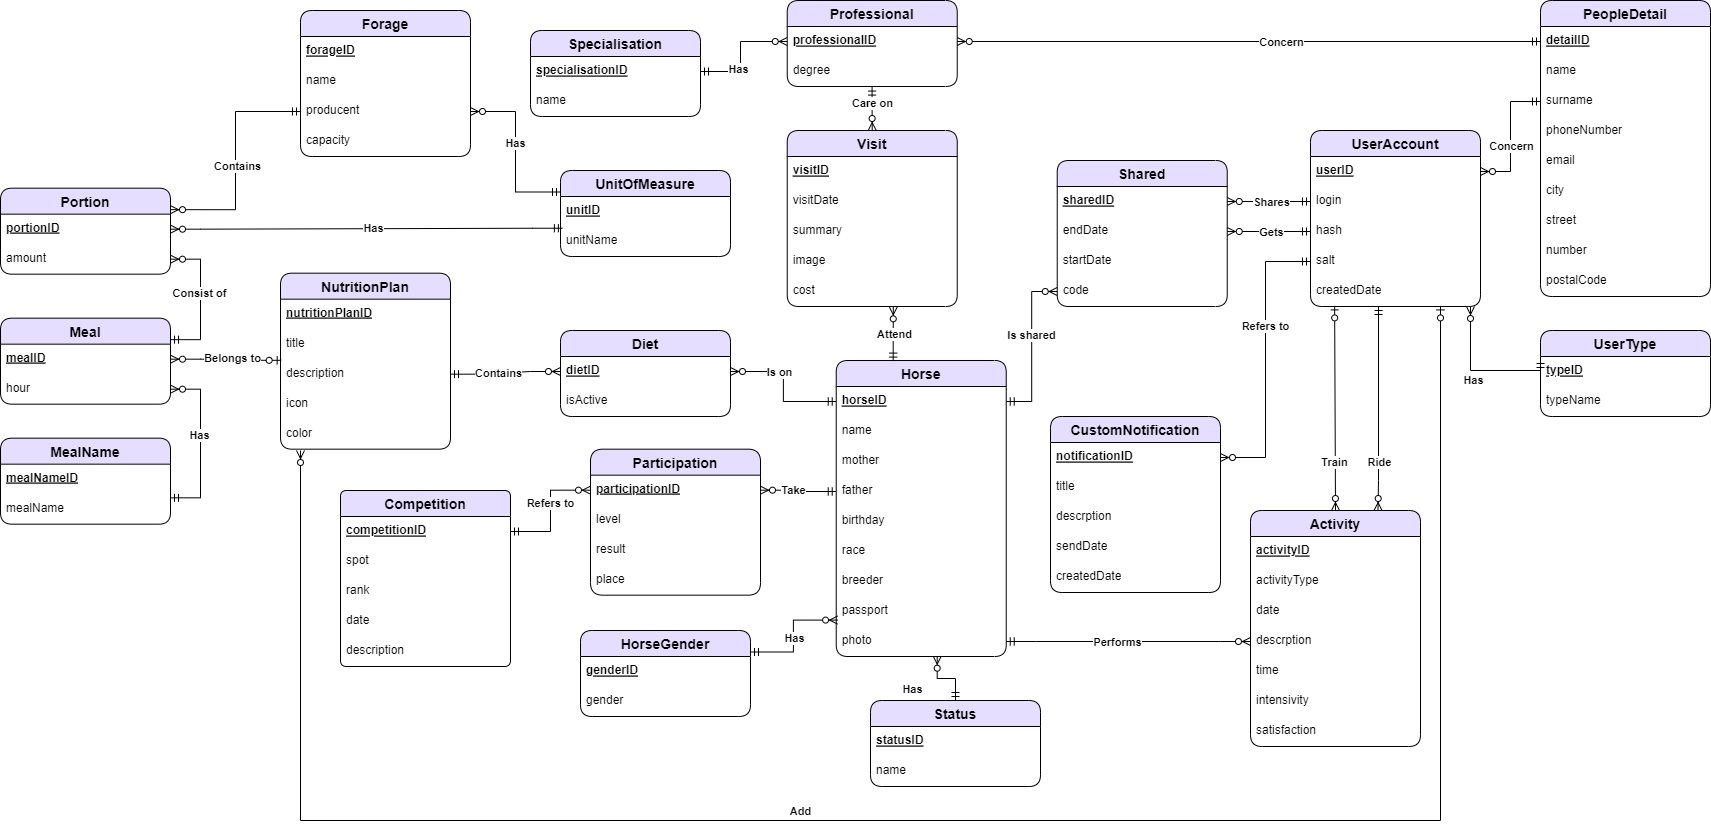
\includegraphics[scale=0.35, angle=-90]{DiagramERD}
		\caption{Diagram ERD}
		\textit{Źródło: Opracowanie własne}
		\label{DiagramERD}
\end{figure}
\section{Model logiczny}
Po stworzeniu modelu konceptualnego, należy przetransformować go do modelu logicznego. Poniżej przedstawiono tabele opisujące schematy relacji oraz znaczenia atrybutów tych relacji.
\begin{enumerate}[start=1,label={\bfseries REL\textbackslash0\arabic*}]
	\item \textbf{Activities\textbackslash ACTIVITY} \\
	Opis schematu relacji znajduje się w tabeli \ref{ActivityRelationSchema}.
	
	\begin{table}[H]
		\caption{Opis schematu relacji Activities}
		\textit{Źródło: Opracowanie własne}
		\label{ActivityRelationSchema}
		\centering
		\begin{tabular}{|c|c|c|c|c|c|c|c|c|c|}
			\hline
			\begin{sideways}Nazwa atrybutu\end{sideways}& 
			\begin{sideways}Dziedzina \end{sideways}& 
			\begin{sideways}Maska \end{sideways}& 
			\begin{sideways}OBL(+) OPC(-)\end{sideways} & 
			\begin{sideways}Wartość domyślna$\ $\end{sideways}& 
			\begin{sideways}Ograniczenia\end{sideways} &
			\begin{sideways}Unikalność \end{sideways}& 
			\begin{sideways}Klucz \end{sideways}& 
			\begin{sideways}Referencje \end{sideways}&
			\begin{sideways}Źródło danych\end{sideways}\\
			\hline
			\textit{activityID} & Integer+ & & + & & & + & PR & &BD\\
			\hline
			\textit{date} & Date & dd-mm-rrrr& + & & & & & &USER\\
			\hline
			\textit{description} & String & & - & & & & & &USER\\
			\hline
			\textit{time} & Integer & & + & & & & & &USER\\
			\hline
			\textit{intensivity}  & Integer+ & & + & & & & & &USER\\
			\hline
			\textit{satisfaction} & Integer+ & & + & & & & & &USER\\
			\hline
			\textit{activityType} & Integer+ & & + & & & & & &USER\\
			\hline
			\textit{userID} & Integer+ & & + & & & &FK&User&BD\\
			\hline	
			\textit{horseID} & Integer+ & & + & & & &FK&Horse&BD\\
			\hline
			\textit{trainerID} & Integer+ & & - & & & &FK&User&BD\\
			\hline		
		\end{tabular}
	\end{table}

	\begin{table}[H]
	\caption{Opis atrybutów relacji Activities}
	\textit{Źródło: Opracowanie własne}
	\label{ActivityAttributeDescription}
	\centering
	\begin{tabular}{|c|c|}
\hline
Nazwa atrybutu & Znaczenie \\
\hline
\textit{activityID} & Unikalne ID aktywności, generowane przez aplikację, klucz główny tabeli. \\
\hline
\textit{date} &  Data wykonywanej aktywności.\\
\hline
\textit{description} & Opis aktywności, dowolne polskie znaki.\\
\hline
\textit{time} & Liczba naturalna, oznaczająca czas trwania wykonywanej aktywności.\\
\hline
\textit{intensivity}  & Liczba naturalna od 0 do 5 oznaczająca poziom intensywności treningu.\\
\hline
\textit{satisfaction} & Liczba naturalna od 0 do 5 oznaczająca poziom satysfakcji z treningu.\\
\hline
\textit{activityType} &  Liczba naturalna oznaczająca typ aktywności.\\
			\hline
\textit{userID} & Indentyfikator użytkownika, który wpisuje aktywność.\\
\hline	
\textit{horseID} & Identyfikator konia, którego dotyczy aktywność.\\
\hline
\textit{trainerID} & Identyfikator użytkownika typu trener, który przeprowadzał trening.\\
\hline
	\end{tabular}
\end{table}

	\item \textbf{Competitions\textbackslash COMPETITION} \\
Opis schematu relacji znajduje się w tabeli \ref{CompetitionsRelationSchema}.
\begin{table}[h!]
	\caption{Opis schematu relacji Competitions}
	\textit{Źródło: Opracowanie własne}
	\label{CompetitionsRelationSchema}
	\centering
	\begin{tabular}{|c|c|c|c|c|c|c|c|c|c|}
		\hline
		\begin{sideways}Nazwa atrybutu\end{sideways}& 
		\begin{sideways}Dziedzina \end{sideways}& 
		\begin{sideways}Maska \end{sideways}& 
		\begin{sideways}OBL(+) OPC(-)\end{sideways} & 
		\begin{sideways}Wartość domyślna$\ $\end{sideways}& 
		\begin{sideways}Ograniczenia\end{sideways} &
		\begin{sideways}Unikalność \end{sideways}& 
		\begin{sideways}Klucz \end{sideways}& 
		\begin{sideways}Referencje \end{sideways}&
		\begin{sideways}Źródło danych\end{sideways}\\
		\hline
		\textit{competitionID} & Integer+ & & + & & & + & PR & &BD\\
		\hline
		\textit{spot} & String & & - & & & & & &USER\\
		\hline
		\textit{rank} & String & & - & & & & & &USER\\
		\hline
		\textit{date} & Date & & + & & & & & &USER\\
		\hline
		\textit{description}  & String & & + & & & & & &USER\\
		\hline		
	\end{tabular}
\end{table}

\begin{table}[H]
	\caption{Opis atrybutów relacji Competitions}
	\textit{Źródło: Opracowanie własne}
	\label{CompetitionsAttributeDescription}
	\centering
	\begin{tabular}{|c|c|}
		\hline
		Nazwa atrybutu & Znaczenie \\
		\hline
		\textit{competitionID} & Unikalny numer ID identyfikujący zawody, generowany przez aplikację.\\
\hline
\textit{spot} & Miejsce, w którym odbędą się zawody.\\
\hline
\textit{rank} & Ranga zawodów np. regionalne/międzynarodowe itp.\\
\hline
\textit{date} & Dzień, w którym odbędą się zawody.\\
\hline
\textit{description}  & Opis zawodów.\\
\hline	
	\end{tabular}
\end{table}
\item \textbf{Notifications\textbackslash NOTIFICATION}
\begin{table}[H]
	\caption{Opis schematu relacji Notifications}
	\textit{Źródło: Opracowanie własne}
	\label{NotificationsRelationSchema}
	\centering
	\begin{tabular}{|c|c|c|c|c|c|c|c|c|c|}
		\hline
		\begin{sideways}Nazwa atrybutu\end{sideways}& 
		\begin{sideways}Dziedzina \end{sideways}& 
		\begin{sideways}Maska \end{sideways}& 
		\begin{sideways}OBL(+) OPC(-)\end{sideways} & 
		\begin{sideways}Wartość domyślna$\ $\end{sideways}& 
		\begin{sideways}Ograniczenia\end{sideways} &
		\begin{sideways}Unikalność \end{sideways}& 
		\begin{sideways}Klucz \end{sideways}& 
		\begin{sideways}Referencje \end{sideways}&
		\begin{sideways}Źródło danych\end{sideways}\\
			\hline
	\textit{notificationID} & Integer+& & + &&&+&PR&&BD\\
	\hline
	\textit{title} & String& & + &&&&&&USER\\
	\hline
	\textit{description}  & String& & + &&&&&&USER\\
	\hline
	\textit{sendDate}  & Date& & + &&&&&&USER\\
	\hline
	\textit{createdDate} & Date& & + &&&&&&USER\\
	\hline
	userID&Integer+& &+&&&&FK&User&BD\\
	\hline
	\end{tabular}
\end{table}

\begin{table}[H]
	\caption{Opis atrybutów relacji Notifiactions}
	\textit{Źródło: Opracowanie własne}
	\label{NotifiactionsAttributeDescription}
	\centering
	\begin{tabular}{|c|c|}
		\hline
		Nazwa atrybutu & Znaczenie \\
		\hline
		\textit{notificationID} & Unikalny numer ID identyfikujący powiadomienie \\
		\hline
		\textit{title} &  Tytuł powiadomienia\\
		\hline
		\textit{description} & Opis pojawiający się na powiadomieniu\\
		\hline
		\textit{sendDate} &  Data i godzina informująca kiedy ma zostać wysłane powiadomienie\\
		\hline
		\textit{createdDate} &  Data i godzina stworzenia powiadomienia\\
		\hline		
		\textit{userID} & Numer ID identyfikujący użytkownika wysyłającego powiadomienie \\
		\hline
	\end{tabular}
\end{table}
\item \textbf{Profesionals\textbackslash PROFESTIONAL}
\begin{table}[H]
	\caption{Opis schematu relacji Profesionals}
	\textit{Źródło: Opracowanie własne}
	\label{ProfesionalsRelationSchema}
	\centering
	\begin{tabular}{|c|c|c|c|c|c|c|c|c|c|}
		\hline
		\begin{sideways}Nazwa atrybutu\end{sideways}& 
		\begin{sideways}Dziedzina \end{sideways}& 
		\begin{sideways}Maska \end{sideways}& 
		\begin{sideways}OBL(+) OPC(-)\end{sideways} & 
		\begin{sideways}Wartość domyślna$\ $\end{sideways}& 
		\begin{sideways}Ograniczenia\end{sideways} &
		\begin{sideways}Unikalność \end{sideways}& 
		\begin{sideways}Klucz \end{sideways}& 
		\begin{sideways}Referencje \end{sideways}&
		\begin{sideways}Źródło danych\end{sideways}\\
		\hline
		\textit{profesionalID}&Integer+&&+&&&+&PR&&BD\\
		\hline
		\textit{degree}&String&&-&&&&&&USER\\
		\hline
		\textit{detailsID}&Integer+&&+&&&&FK&Details&BD\\
		\hline
		\textit{specialisationID}&Integer+&&+&&&&FK&Sepcialisation&BD\\
		\hline
	\end{tabular}
\end{table}

\begin{table}[H]
	\caption{Opis atrybutów relacji Profesionals}
	\textit{Źródło: Opracowanie własne}
	\label{ProfesionalsAttributeDescription}
	\centering
	\begin{tabular}{|c|c|}
		\hline
		Nazwa atrybutu & Znaczenie \\
			\hline
		\textit{profesionalID}& Unikalny numer ID identyfikujący profesjonalistę\\
		\hline
		\textit{degree}& Stopien naukowy profesjonalisty\\
		\hline
		\textit{detailsID}& Numer ID identyfikujący dane personalne profesjonalistę\\
		\hline
		\textit{specialisationID}&Numer ID identyfikujący specjalizacje profesjonalisty\\
		\hline
	\end{tabular}
\end{table}
\item \textbf{Specialisations\textbackslash SPECIALISATION}
\begin{table}[H]
	\caption{Opis schematu relacji Specialisations}
	\textit{Źródło: Opracowanie własne}
	\label{SpecialisationsRelationSchema}
	\centering
	\begin{tabular}{|c|c|c|c|c|c|c|c|c|c|}
		\hline
		\begin{sideways}Nazwa atrybutu\end{sideways}& 
		\begin{sideways}Dziedzina \end{sideways}& 
		\begin{sideways}Maska \end{sideways}& 
		\begin{sideways}OBL(+) OPC(-)\end{sideways} & 
		\begin{sideways}Wartość domyślna$\ $\end{sideways}& 
		\begin{sideways}Ograniczenia\end{sideways} &
		\begin{sideways}Unikalność \end{sideways}& 
		\begin{sideways}Klucz \end{sideways}& 
		\begin{sideways}Referencje \end{sideways}&
		\begin{sideways}Źródło danych\end{sideways}\\
		\hline
		\textit{specialisationID}&Integer+&&+&&&+&PK&&BD\\
		\hline
		\textit{name}&String&&+&&&&&&USER\\
		\hline
	\end{tabular}
\end{table}

\begin{table}[H]
	\caption{Opis atrybutów relacji Profesionals}
	\textit{Źródło: Opracowanie własne}
	\label{SpecialisationsAttributeDescription}
	\centering
	\begin{tabular}{|c|c|}
		\hline
		Nazwa atrybutu & Znaczenie \\
		\hline
		\textit{specialisationID}& Unikalny numer ID identyfikujący specjalizację.\\
		\hline
		\textit{name}& Nazwa specjalizacji\\
		\hline
	\end{tabular}
\end{table}
\item \textbf{Diets\textbackslash DIET}
\begin{table}[H]
	\caption{Opis schematu relacji Diets}
	\textit{Źródło: Opracowanie własne}
	\label{DietsRelationSchema}
	\centering
	\begin{tabular}{|c|c|c|c|c|c|c|c|c|c|}
		\hline
		\begin{sideways}Nazwa atrybutu\end{sideways}& 
		\begin{sideways}Dziedzina \end{sideways}& 
		\begin{sideways}Maska \end{sideways}& 
		\begin{sideways}OBL(+) OPC(-)\end{sideways} & 
		\begin{sideways}Wartość domyślna$\ $\end{sideways}& 
		\begin{sideways}Ograniczenia\end{sideways} &
		\begin{sideways}Unikalność \end{sideways}& 
		\begin{sideways}Klucz \end{sideways}& 
		\begin{sideways}Referencje \end{sideways}&
		\begin{sideways}Źródło danych\end{sideways}\\
		\hline
		 \textit{dietID}&Integer+&&+&&&+&PR&&BD\\
		 \hline
		 \textit{isActive}&Boolean&&+&true&&&&&\\
		 \hline
		 \textit{horseID}&Integer+&&+&&&&FK&Horse&BD\\
		 \hline
		 \textit{nutritionPlanID}&Integer+&&+&&&&FK&NutritionPlan&BD\\
		 \hline
	\end{tabular}
\end{table}

\begin{table}[H]
	\caption{Opis atrybutów relacji Diets}
	\textit{Źródło: Opracowanie własne}
	\label{DietsAttributeDescription}
	\centering
	\begin{tabular}{|c|c|}
		\hline
		Nazwa atrybutu & Znaczenie \\
				\hline
		\textit{dietID}& Unikalny numer ID identyfikujący daną dietę\\
		\hline
		\textit{isActive}& Zmienna przyjmująca wartości true/false \\
		\hline
		\textit{horseID}& Numer ID identyfikujący konia\\
		\hline
		\textit{nutritionPlanID}& Numer ID identyfikujący plan żywienia\\
		\hline
	\end{tabular}
\end{table}
\item \textbf{Portions\textbackslash PORTION} 
\begin{table}[H]
	\caption{Opis schematu relacji Portions}
	\textit{Źródło: Opracowanie własne}
	\label{PortionsRelationSchema}
	\centering
	\begin{tabular}{|c|c|c|c|c|c|c|c|c|c|}
		\hline
		\begin{sideways}Nazwa atrybutu\end{sideways}& 
		\begin{sideways}Dziedzina \end{sideways}& 
		\begin{sideways}Maska \end{sideways}& 
		\begin{sideways}OBL(+) OPC(-)\end{sideways} & 
		\begin{sideways}Wartość domyślna$\ $\end{sideways}& 
		\begin{sideways}Ograniczenia\end{sideways} &
		\begin{sideways}Unikalność \end{sideways}& 
		\begin{sideways}Klucz \end{sideways}& 
		\begin{sideways}Referencje \end{sideways}&
		\begin{sideways}Źródło danych\end{sideways}\\
		\hline
		\textit{portionID}&Integer+&&+&&&+&PR&&BD\\		
		\hline
		\textit{amount}&Float+&&+&1&0<&&&&USER\\
		\hline
	\end{tabular}
\end{table}

\begin{table}[H]
	\caption{Opis atrybutów relacji Portions}
	\textit{Źródło: Opracowanie własne}
	\label{PortionsAttributeDescription}
	\centering
	\begin{tabular}{|c|c|}
		\hline
		Nazwa atrybutu & Znaczenie \\
				\hline
		\textit{portionID}& Unikalny numer ID identyfikujący porcję jedzenia dla konia \\		
		\hline
		\textit{amount}& Ilość jedzenia w porcji\\
		\hline
	\end{tabular}
\end{table}
\item \textbf{Forges\textbackslash FORAGE} (\textit{\underline{forageID}, name, producent, capacity})
\begin{table}[H]
	\caption{Opis schematu relacji Forges}
	\textit{Źródło: Opracowanie własne}
	\label{ForgesRelationSchema}
	\centering
	\begin{tabular}{|c|c|c|c|c|c|c|c|c|c|}
		\hline
		\begin{sideways}Nazwa atrybutu\end{sideways}& 
		\begin{sideways}Dziedzina \end{sideways}& 
		\begin{sideways}Maska \end{sideways}& 
		\begin{sideways}OBL(+) OPC(-)\end{sideways} & 
		\begin{sideways}Wartość domyślna$\ $\end{sideways}& 
		\begin{sideways}Ograniczenia\end{sideways} &
		\begin{sideways}Unikalność \end{sideways}& 
		\begin{sideways}Klucz \end{sideways}& 
		\begin{sideways}Referencje \end{sideways}&
		\begin{sideways}Źródło danych\end{sideways}\\
		\hline
		\textit{forageID}&Integer+&&+&&&+&PR&&BD\\		
		\hline		
		\textit{name}&String&&+&&&&&&USER\\		
		\hline
		\textit{producent}&String&&+&&&&&&USER\\		
		\hline		
		\textit{capacity}&String&&+&&&&&&USER\\		
		\hline
		\textit{unitID}&Integer+&&+&&&&FK&UnitOfMeasure&BD\\
		\hline
	\end{tabular}
\end{table}

\begin{table}[H]
	\caption{Opis atrybutów relacji Forges}
	\textit{Źródło: Opracowanie własne}
	\label{ForgesAttributeDescription}
	\centering
	\begin{tabular}{|c|c|}
		\hline
		Nazwa atrybutu & Znaczenie \\
		\hline
		\textit{forageID}&Unikalny numer ID identyfikujący paszę\\		
		\hline		
		\textit{name}&Nazwa paszy\\		
		\hline
		\textit{producent}&Nazwa producenta paszy\\		
		\hline		
		\textit{capacity}&Liczba naturalna oznaczająca ilość paszy w jednej paczce paszy\\		
		\hline
		\textit{unitID}& Numer ID identyfikujący jednostkę miary\\
		\hline
	\end{tabular}
\end{table}
\item \textbf{Horses\textbackslash HORSE} 
\begin{table}[H]
	\caption{Opis schematu relacji Horses}
	\textit{Źródło: Opracowanie własne}
	\label{HorsesRelationSchema}
	\centering
	\begin{tabular}{|c|c|c|c|c|c|c|c|c|c|}
		\hline
		\begin{sideways}Nazwa atrybutu\end{sideways}& 
		\begin{sideways}Dziedzina \end{sideways}& 
		\begin{sideways}Maska \end{sideways}& 
		\begin{sideways}OBL(+) OPC(-)\end{sideways} & 
		\begin{sideways}Wartość domyślna$\ $\end{sideways}& 
		\begin{sideways}Ograniczenia\end{sideways} &
		\begin{sideways}Unikalność \end{sideways}& 
		\begin{sideways}Klucz \end{sideways}& 
		\begin{sideways}Referencje \end{sideways}&
		\begin{sideways}Źródło danych\end{sideways}\\
		\hline
		\textit{horseID}&Integer+&&+&&&+&PR&&BD\\		
		\hline			
		\textit{name}&Integer+&&+&&&&&&USER\\		
		\hline			
		\textit{mother}&Integer+&&+&&&&&&USER\\		
		\hline			
		\textit{father}&Integer+&&+&&&&&&USER\\		
		\hline			
		\textit{birthday}&Date&&+&&&&&&USER\\		
		\hline			
		\textit{race}&String&&+&&&&&&USER\\		
		\hline			
		\textit{breeder}&String&&+&&&&&&USER\\		
		\hline			
		\textit{passport}&String&&+&&&&&&USER\\		
		\hline			
		\textit{photo}&String&&+&&&&&&USER\\		
		\hline		
		\textit{statusID}&Integer+&&+&&&&FK&Status&USER\\		
		\hline
		\textit{genderID}&Integer+&&+&&&&FK&HorseGender&USER\\		
		\hline
	\end{tabular}
\end{table}

\begin{table}[H]
	\caption{Opis atrybutów relacji Horses}
	\textit{Źródło: Opracowanie własne}
	\label{HorsesAttributeDescription}
	\centering
	\begin{tabular}{|c|c|}
		\hline
		Nazwa atrybutu & Znaczenie \\
		\hline
		\textit{horseID}&Unikalny numer ID identyfikujący konia\\		
		\hline			
		\textit{name}& Imię konia\\		
		\hline			
		\textit{mother}& Imię matki konia\\		
		\hline			
		\textit{father}& Imię ojca konia\\		
		\hline			
		\textit{birthday}& Data urodzenia\\		
		\hline			
		\textit{race}& Rasa konia\\		
		\hline			
		\textit{breeder}& Nazwa hodowli lub imię i nazwisko hodowcy\\		
		\hline			
		\textit{passport}& Numer paszportu\\		
		\hline			
		\textit{photo}& URL zdjęcia\\		
		\hline		
		\textit{statusID}& Numer ID identyfikujący status konia\\		
		\hline
		\textit{genderID}&Numer ID identyfikujący płeć konia\\		
		\hline
	\end{tabular}
\end{table}
\end{enumerate}
\begin{enumerate}[start=10,label={\bfseries REL\textbackslash\arabic*}]
	\item \textbf{HorseGenders\textbackslash HORSEGENDER} 
	\begin{table}[H]
		\caption{Opis schematu relacji HorseGenders}
		\textit{Źródło: Opracowanie własne}
		\label{HorseGendersRelationSchema}
		\centering
		\begin{tabular}{|c|c|c|c|c|c|c|c|c|c|}
			\hline
			\begin{sideways}Nazwa atrybutu\end{sideways}& 
			\begin{sideways}Dziedzina \end{sideways}& 
			\begin{sideways}Maska \end{sideways}& 
			\begin{sideways}OBL(+) OPC(-)\end{sideways} & 
			\begin{sideways}Wartość domyślna$\ $\end{sideways}& 
			\begin{sideways}Ograniczenia\end{sideways} &
			\begin{sideways}Unikalność \end{sideways}& 
			\begin{sideways}Klucz \end{sideways}& 
			\begin{sideways}Referencje \end{sideways}&
			\begin{sideways}Źródło danych\end{sideways}\\
			\hline
			\textit{genderID}&Integer+&&+&&&+&PK&&USER\\	
			\hline
			\textit{gender}&String&&&&&&&&USER\\
			\hline		
		\end{tabular}
	\end{table}
	
	\begin{table}[H]
		\caption{Opis atrybutów relacji HorseGenders}
		\textit{Źródło: Opracowanie własne}
		\label{HorseGendersAttributeDescription}
		\centering
		\begin{tabular}{|c|c|}
			\hline
			Nazwa atrybutu & Znaczenie \\
			\hline
			\textit{genderID}& Unikalny numer ID identyfikujący płeć konia\\	
			\hline
			\textit{gender}& Nazwa płci\\
			\hline
		\end{tabular}
	\end{table}
	\item \textbf{Status\textbackslash STATUS} 
	\begin{table}[H]
		\caption{Opis schematu relacji Specialisations}
		$\ $
		\textit{Źródło: Opracowanie własne}
		\label{StatusRelationSchema}
		\centering
		\begin{tabular}{|c|c|c|c|c|c|c|c|c|c|}
			\hline
			\begin{sideways}Nazwa atrybutu\end{sideways}& 
			\begin{sideways}Dziedzina \end{sideways}& 
			\begin{sideways}Maska \end{sideways}& 
			\begin{sideways}OBL(+) OPC(-)\end{sideways} & 
			\begin{sideways}Wartość domyślna$\ $\end{sideways}& 
			\begin{sideways}Ograniczenia\end{sideways} &
			\begin{sideways}Unikalność \end{sideways}& 
			\begin{sideways}Klucz \end{sideways}& 
			\begin{sideways}Referencje \end{sideways}&
			\begin{sideways}Źródło danych\end{sideways}\\
			\hline
			\textit{statusID}&Integer+&&+&&&+&PK&&BD\\	
			\hline			
			\textit{name}&String&&+&&&&&&USER\\	
			\hline
		\end{tabular}
	\end{table}
	
	\begin{table}[H]
		\caption{Opis atrybutów relacji Status}
		\textit{Źródło: Opracowanie własne}
		\label{StatusAttributeDescription}
		\centering
		\begin{tabular}{|c|c|}
			\hline
			Nazwa atrybutu & Znaczenie \\
			\hline
		    \textit{statusID}&Unikalny numer ID identyfikujący status konia bądź użytkownika\\	
			\hline			
			\textit{name}& Nazwa statusu\\	
			\hline
		\end{tabular}
	\end{table}
	\item \textbf{MealNames\textbackslash MEALNAME} 
	\begin{table}[H]
		\caption{Opis schematu relacji MealNames}
		\textit{Źródło: Opracowanie własne}
		\label{MealNamesRelationSchema}
		\centering
		\begin{tabular}{|c|c|c|c|c|c|c|c|c|c|}
			\hline
			\begin{sideways}Nazwa atrybutu\end{sideways}& 
			\begin{sideways}Dziedzina \end{sideways}& 
			\begin{sideways}Maska \end{sideways}& 
			\begin{sideways}OBL(+) OPC(-)\end{sideways} & 
			\begin{sideways}Wartość domyślna$\ $\end{sideways}& 
			\begin{sideways}Ograniczenia\end{sideways} &
			\begin{sideways}Unikalność \end{sideways}& 
			\begin{sideways}Klucz \end{sideways}& 
			\begin{sideways}Referencje \end{sideways}&
			\begin{sideways}Źródło danych\end{sideways}\\
			\hline			
			\textit{mealNameID}&Integer+&&+&&&+&PK&&BD\\	
			\hline			
			\textit{mealName}&String&&+&&&&&&USER\\	
			\hline
		\end{tabular}
	\end{table}
	
	\begin{table}[H]
		\caption{Opis atrybutów relacji MealNames}
		\textit{Źródło: Opracowanie własne}
		\label{MealNamesAttributeDescription}
		\centering
		\begin{tabular}{|c|c|}
			\hline
			Nazwa atrybutu & Znaczenie \\			
			\hline			
			\textit{mealNameID}&Unikatowy numer ID identyfikujący nazwę posiłku\\	
			\hline			
			\textit{mealName}& Nazwa posiłku\\	
			\hline
		\end{tabular}
	\end{table}
	\item \textbf{NutritionPlans\textbackslash NUTRITIONPLAN} \begin{table}[H]
		\caption{Opis schematu relacji NutritionPlans}
		\textit{Źródło: Opracowanie własne}
		\label{NutritionPlansRelationSchema}
		\centering
		\begin{tabular}{|c|c|c|c|c|c|c|c|c|c|}
			\hline
			\begin{sideways}Nazwa atrybutu\end{sideways}& 
			\begin{sideways}Dziedzina \end{sideways}& 
			\begin{sideways}Maska \end{sideways}& 
			\begin{sideways}OBL(+) OPC(-)\end{sideways} & 
			\begin{sideways}Wartość domyślna$\ $\end{sideways}& 
			\begin{sideways}Ograniczenia\end{sideways} &
			\begin{sideways}Unikalność \end{sideways}& 
			\begin{sideways}Klucz \end{sideways}& 
			\begin{sideways}Referencje \end{sideways}&
			\begin{sideways}Źródło danych\end{sideways}\\
			\hline			
			\textit{nutritionPlanID}&Integer+&&+&&&+&PK&&BD\\	
			\hline			
			\textit{title}&String&&+&&&&&&USER\\	
			\hline			
			\textit{description}&String&&-&&&&&&USER\\	
			\hline			
			\textit{icon}&Integer+&&+&1&&&&&USER\\	
			\hline
		\end{tabular}
	\end{table}
	
	\begin{table}[H]
		\caption{Opis atrybutów relacji NutritionPlans}
		\textit{Źródło: Opracowanie własne}
		\label{NutritionPlansAttributeDescription}
		\centering
		\begin{tabular}{|c|c|}
			\hline
			Nazwa atrybutu & Znaczenie \\
			\hline			
			\textit{nutritionPlanID}& Unikatowy numer ID identyfikujący plan żywienia\\	
			\hline			
			\textit{title}&Tytuł planu żywienia\\	
			\hline			
			\textit{description}&Opis planu żywienia\\	
			\hline			
			\textit{icon}&Id ikonki wyświetlanej koło planu żywienia\\	
			\hline
		\end{tabular}
	\end{table}
	\item \textbf{PeopleDetails\textbackslash PEOPLEDETIALS}
	 \begin{table}[H]
		\caption{Opis schematu relacji PeopleDetails}
		\textit{Źródło: Opracowanie własne}
		\label{PeopleDetailsRelationSchema}
		\centering
		\begin{tabular}{|c|c|c|c|c|c|c|c|c|c|}
			\hline
			\begin{sideways}Nazwa atrybutu\end{sideways}& 
			\begin{sideways}Dziedzina \end{sideways}& 
			\begin{sideways}Maska \end{sideways}& 
			\begin{sideways}OBL(+) OPC(-)\end{sideways} & 
			\begin{sideways}Wartość domyślna$\ $\end{sideways}& 
			\begin{sideways}Ograniczenia\end{sideways} &
			\begin{sideways}Unikalność \end{sideways}& 
			\begin{sideways}Klucz \end{sideways}& 
			\begin{sideways}Referencje \end{sideways}&
			\begin{sideways}Źródło danych\end{sideways}\\
			\hline			
			\textit{detailsID}&Integer+&&+&&&+&PK&&BD\\	
			\hline			
			\textit{name}&String&&+&&&&&&USER\\	
			\hline			
			\textit{surname}&String&&-&&&&&&USER\\	
			\hline			
			\textit{phonNumber}&String&+\_\_\_\_\_\_\_\_\_\_\_&+&&&&&&USER\\	
			\hline			
			\textit{email}&Integer+&\underline{\qquad\qquad}@\underline{\qquad}&+&&&&&&USER\\	
			\hline			
			\textit{city}&Integer+&&+&&&&&&USER\\	
			\hline			
			\textit{street}&Integer+&&+&&&&&&USER\\	
			\hline			
			\textit{number}&Integer+&&+&&&&&&USER\\	
			\hline
		\end{tabular}
	\end{table}
	
	\begin{table}[H]
		\caption{Opis atrybutów relacji PeopleDetails}
		\textit{Źródło: Opracowanie własne}
		\label{PeopleDetailsAttributeDescription}
		\centering
		\begin{tabular}{|c|c|}
			\hline
			Nazwa atrybutu & Znaczenie \\
			\hline			
			\textit{detailsID}& Unikalny numer ID identyfikujący detale ludzi\\	
			\hline			
			\textit{name}& Imie \\	
			\hline			
			\textit{surname}& Nazwisko\\	
			\hline			
			\textit{phonNumber}& Numer telefonu\\	
			\hline			
			\textit{email}& Adres e-mail\\	
			\hline			
			\textit{city}& Miasto \\	
			\hline			
			\textit{street}& Ulica\\	
			\hline			
			\textit{number}& Numer domu\\	
			\hline
		\end{tabular}
	\end{table}
	\item \textbf{Participations\textbackslash PARTICIPATION} 
	\begin{table}[H]
		\caption{Opis schematu relacji Participations}
		\textit{Źródło: Opracowanie własne}
		\label{ParticipationsRelationSchema}
		\centering
		\begin{tabular}{|c|c|c|c|c|c|c|c|c|c|}
			\hline
			\begin{sideways}Nazwa atrybutu\end{sideways}& 
			\begin{sideways}Dziedzina \end{sideways}& 
			\begin{sideways}Maska \end{sideways}& 
			\begin{sideways}OBL(+) OPC(-)\end{sideways} & 
			\begin{sideways}Wartość domyślna$\ $\end{sideways}& 
			\begin{sideways}Ograniczenia\end{sideways} &
			\begin{sideways}Unikalność \end{sideways}& 
			\begin{sideways}Klucz \end{sideways}& 
			\begin{sideways}Referencje \end{sideways}&
			\begin{sideways}Źródło danych\end{sideways}\\
			\hline			
			\textit{ParticipationID}&Integer+&&+&&&+&PK&&BD\\	
			\hline			
			\textit{level}&Integer+&&+&&&&&&BD\\	
			\hline			
			\textit{result}&String&&+&&&&&&USER\\	
			\hline			
			\textit{place}&String&&+&&&&&&USER\\	
			\hline			
			\textit{competitionID}&Integer+&&+&&&&&&BD\\	
			\hline
			\textit{horseID}&Integer+&&+&&&&&&BD\\	
			\hline
		\end{tabular}
	\end{table}
	
	\begin{table}[H]
		\caption{Opis atrybutów relacji Participations}
		\textit{Źródło: Opracowanie własne}
		\label{ParticipationsAttributeDescription}
		\centering
		\begin{tabular}{|c|c|}
			\hline
			Nazwa atrybutu & Znaczenie \\
			\hline			
			\textit{ParticipationID}&Unikalny numer ID identyfikujący start w zawodach.\\	
			\hline			
			\textit{level}&Poziom konkursu, w którym koń brał udział\\	
			\hline			
			\textit{result}&Wynik z danego konkursu\\	
			\hline			
			\textit{place}&Miejsce uzyskane w danym konkursie\\	
			\hline			
			\textit{competitionID}& Numer ID zawodów, w których koń bierze udział\\	
			\hline
			\textit{horseID}&Numer ID konia biorącego udział w zawodach\\	
			\hline
		\end{tabular}
	\end{table}
	\item \textbf{Shareds\textbackslash SHARED} 
	\begin{table}[H]
		\caption{Opis schematu relacji Shareds}
		\textit{Źródło: Opracowanie własne}
		\label{SharedsRelationSchema}
		\centering
		\begin{tabular}{|c|c|c|c|c|c|c|c|c|c|}
			\hline
			\begin{sideways}Nazwa atrybutu\end{sideways}& 
			\begin{sideways}Dziedzina \end{sideways}& 
			\begin{sideways}Maska \end{sideways}& 
			\begin{sideways}OBL(+) OPC(-)\end{sideways} & 
			\begin{sideways}Wartość domyślna$\ $\end{sideways}& 
			\begin{sideways}Ograniczenia\end{sideways} &
			\begin{sideways}Unikalność \end{sideways}& 
			\begin{sideways}Klucz \end{sideways}& 
			\begin{sideways}Referencje \end{sideways}&
			\begin{sideways}Źródło danych\end{sideways}\\
			\hline			
			\textit{sharedID}&Integer+&&+&&&+&PK&&BD\\
			\hline			
			\textit{code}&String&&+&&&&&&USER\\				
			\hline			
			\textit{endDate}&Date&&+&&&&&&USER\\
			\hline			
			\textit{startDate}&Date&&+&&&&&&USER\\				
			\hline
			\textit{horseID}&Integer+&&+&&&&&&USER\\				
			\hline
			\textit{userSharedID}&Integer+&&+&&&&FK&USER&BD\\				
			\hline
			\textit{userScanID}&Integer+&&+&&&&FK&USER&BD\\	
			\hline
		\end{tabular}
	\end{table}
	
	\begin{table}[H]
		\caption{Opis atrybutów relacji Shareds}
		\textit{Źródło: Opracowanie własne}
		\label{SharedsAttributeDescription}
		\centering
		\begin{tabular}{|c|c|}
			\hline
			Nazwa atrybutu & Znaczenie \\
			\hline			
			\textit{sharedID}&Unikalny numer ID identyfikujący pojedyncze udostępnienie \\
			& konia między dwoma użytkownikami\\
			\hline			
			\textit{code}& Kod Qr dzięki któremu użytkownicy mogą udostępniać między sobą konie.\\				
			\hline			
			\textit{endDate}& Data kończąca udostępnianie\\
			\hline			
			\textit{startDate}& Data od której koń będzie udostępniony\\				
			\hline
			\textit{horseID}&Numer ID identyfikujący udostępnianego konia\\				
			\hline
			\textit{userSharedID}& Numer ID identyfikujący użytkownika, który udostępnia konia \\				
			\hline
			\textit{userScanID}&Numer ID identyfikujący użytkownika, któremu zostanie udostępniony koń\\	
			\hline
		\end{tabular}
	\end{table}
	\item \textbf{UnitOfmeasures\textbackslash UNITOFMEASURE}
	 \begin{table}[H]
		\caption{Opis schematu relacji UnitOfmeasures}
		\textit{Źródło: Opracowanie własne}
		\label{UnitOfmeasuresRelationSchema}
		\centering
		\begin{tabular}{|c|c|c|c|c|c|c|c|c|c|}
			\hline
			\begin{sideways}Nazwa atrybutu\end{sideways}& 
			\begin{sideways}Dziedzina \end{sideways}& 
			\begin{sideways}Maska \end{sideways}& 
			\begin{sideways}OBL(+) OPC(-)\end{sideways} & 
			\begin{sideways}Wartość domyślna$\ $\end{sideways}& 
			\begin{sideways}Ograniczenia\end{sideways} &
			\begin{sideways}Unikalność \end{sideways}& 
			\begin{sideways}Klucz \end{sideways}& 
			\begin{sideways}Referencje \end{sideways}&
			\begin{sideways}Źródło danych\end{sideways}\\
			\hline
			\textit{unitID}&Integer+&&+&&&+&&&BD\\	
			\hline
			\textit{unitName}&String&&+&&&&&&USER\\	
			\hline
		\end{tabular}
	\end{table}
	
	\begin{table}[H]
		\caption{Opis atrybutów relacji UnitOfmeasures}
		\textit{Źródło: Opracowanie własne}
		\label{UnitOfmeasuresAttributeDescription}
		\centering
		\begin{tabular}{|c|c|}
			\hline
			Nazwa atrybutu & Znaczenie \\
						\hline
			\textit{unitID}&Unikalny numer ID identyfikujący jednostkę miary\\	
			\hline
			\textit{unitName}&Nazwa jednostki miary\\	
			\hline
		\end{tabular}
	\end{table}
	\item \textbf{UserAccounts\textbackslash USERACCOUNT}
	\begin{table}[H]
		\caption{Opis schematu relacji UserAccounts}
		\textit{Źródło: Opracowanie własne}
		\label{UserAccountsRelationSchema}
		\centering
		\begin{tabular}{|c|c|c|c|c|c|c|c|c|c|}
			\hline
			\begin{sideways}Nazwa atrybutu\end{sideways}& 
			\begin{sideways}Dziedzina \end{sideways}& 
			\begin{sideways}Maska \end{sideways}& 
			\begin{sideways}OBL(+) OPC(-)\end{sideways} & 
			\begin{sideways}Wartość domyślna$\ $\end{sideways}& 
			\begin{sideways}Ograniczenia\end{sideways} &
			\begin{sideways}Unikalność \end{sideways}& 
			\begin{sideways}Klucz \end{sideways}& 
			\begin{sideways}Referencje \end{sideways}&
			\begin{sideways}Źródło danych\end{sideways}\\
			\hline
			\textit{userID}&Integer+&&+&&&+&PK&&BD\\	
			\hline
			\textit{accountLogin}&String&&+&&&+&&&USER\\	
			\hline			
			\textit{hash}&String&&+&&&&&&USER\\	
			\hline			
			\textit{salt}&String&&+&&&&&&USER\\	
			\hline			
			\textit{createdDateTime}&Datetime&&+&&&&&&USER\\	
			\hline			
			\textit{typeID}&Integer+&&+&&&&FK&UserTypes&BD\\	
			\hline			
			\textit{detailsID}&Integer+&&+&&&&FK&PeopleDetails&BD\\	
			\hline
		\end{tabular}
	\end{table}
	
	\begin{table}[H]
		\caption{Opis atrybutów relacji UserAccounts}
		\textit{Źródło: Opracowanie własne}
		\label{UserAccountsAttributeDescription}
		\centering
		\begin{tabular}{|c|c|}
			\hline
			Nazwa atrybutu & Znaczenie \\
			\hline
			\textit{userID}&Unikalny numer ID identyfikujący użytkownika \\	
			\hline
			\textit{accountLogin}&Login użytkownika\\	
			\hline			
			\textit{hash}&Hash powstający z hasła użytkownika\\	
			\hline			
			\textit{salt}& Do hasła użytkownika\\	
			\hline			
			\textit{createdDateTime}& Data utworzenia konta\\	
			\hline			
			\textit{typeID}&Numer identyfikujący typ użytkownika\\	
			\hline			
			\textit{detailsID}&Numer identyfikujący detale osobowe użytkownika\\	
			\hline
		\end{tabular}
	\end{table}
	\item \textbf{UserTypes\textbackslash USERTYPE}
	\begin{table}[H]
		\caption{Opis schematu relacji UserTypes}
		\textit{Źródło: Opracowanie własne}
		\label{UserTypesRelationSchema}
		\centering
		\begin{tabular}{|c|c|c|c|c|c|c|c|c|c|}
			\hline
			\begin{sideways}Nazwa atrybutu\end{sideways}& 
			\begin{sideways}Dziedzina \end{sideways}& 
			\begin{sideways}Maska \end{sideways}& 
			\begin{sideways}OBL(+) OPC(-)\end{sideways} & 
			\begin{sideways}Wartość domyślna$\ $\end{sideways}& 
			\begin{sideways}Ograniczenia\end{sideways} &
			\begin{sideways}Unikalność \end{sideways}& 
			\begin{sideways}Klucz \end{sideways}& 
			\begin{sideways}Referencje \end{sideways}&
			\begin{sideways}Źródło danych\end{sideways}\\
			\hline
			\textit{userTypeID}&Integer+&&+&&&+&PK&&BD\\	
			\hline
			\textit{typeName}&String&&+&&&&&&USER\\	
			\hline			
		\end{tabular}
	\end{table}
	
	\begin{table}[H]
		\caption{Opis atrybutów relacji UserTypes}
		\textit{Źródło: Opracowanie własne}
		\label{UserTypesAttributeDescription}
		\centering
		\begin{tabular}{|c|c|}
			\hline
			Nazwa atrybutu & Znaczenie \\
			\hline
			\textit{userTypeID}&Unikalny numer ID identyfikujący typ użytkownika\\	
			\hline
			\textit{typeName}& Nazwa typu użytkownika\\	
			\hline	
		\end{tabular}
	\end{table}
	\item \textbf{Visits\textbackslash VISIT} 
	\begin{table}[H]
		\caption{Opis schematu relacji Visits}
		\textit{Źródło: Opracowanie własne}
		\label{VisitsRelationSchema}
		\centering
		\begin{tabular}{|c|c|c|c|c|c|c|c|c|c|}
			\hline
			\begin{sideways}Nazwa atrybutu\end{sideways}& 
			\begin{sideways}Dziedzina \end{sideways}& 
			\begin{sideways}Maska \end{sideways}& 
			\begin{sideways}OBL(+) OPC(-)\end{sideways} & 
			\begin{sideways}Wartość domyślna$\ $\end{sideways}& 
			\begin{sideways}Ograniczenia\end{sideways} &
			\begin{sideways}Unikalność \end{sideways}& 
			\begin{sideways}Klucz \end{sideways}& 
			\begin{sideways}Referencje \end{sideways}&
			\begin{sideways}Źródło danych\end{sideways}\\
			\hline
			\textit{careID}&Integer+&&+&&&+&PK&&BD\\	
			\hline
			\textit{cost}&Float&&+&&&&&&USER\\	
			\hline	
			\textit{summary}&String&&-&&&&&&USER\\	
			\hline	
			\textit{image}&String&&-&&&&&&USER\\	
			\hline	
			\textit{visitDate}&Date&&+&&&&&&USER\\	
			\hline			
			\textit{horseID}&Integer+&&+&&&&FK&Horse&DB\\	
			\hline			
			\textit{professionalID}&Integer+&&+&&&&FK&Professional&DB\\	
			\hline
		\end{tabular}
	\end{table}
	
	\begin{table}[H]
		\caption{Opis atrybutów relacji Visits}
		\textit{Źródło: Opracowanie własne}
		\label{VisitsAttributeDescription}
		\centering
		\begin{tabular}{|c|c|}
			\hline
			Nazwa atrybutu & Znaczenie \\
						\hline
			\textit{visitID}&Unikalny numer ID identyfikujący wizytę\\	
			\hline	
			\textit{visitDate}& Data wizyty\\	
			\hline	
			\textit{summary}& Podsumowanie wizyty, opis przepisanych leków i innych zaleceń\\	
			\hline	
			\textit{image}& Obraz z wizyty\\	
			\hline
			\textit{cost}&Cena wizyty\\	
			\hline			
			\textit{horseID}&Numer ID identyfikujący konia\\	
			\hline			
			\textit{professionalID}&Numer ID identyfikujący profesjonalistę, który przeprowadza wizytę\\	
			\hline
		\end{tabular}
	\end{table}
	\item \textbf{Meals\textbackslash MEAL} 
	\begin{table}[H]
		\caption{Opis schematu relacji Meals}
		\textit{Źródło: Opracowanie własne}
		\label{MealsRelationSchema}
		\centering
		\begin{tabular}{|c|c|c|c|c|c|c|c|c|c|}
			\hline
			\begin{sideways}Nazwa atrybutu\end{sideways}& 
			\begin{sideways}Dziedzina \end{sideways}& 
			\begin{sideways}Maska \end{sideways}& 
			\begin{sideways}OBL(+) OPC(-)\end{sideways} & 
			\begin{sideways}Wartość domyślna$\ $\end{sideways}& 
			\begin{sideways}Ograniczenia\end{sideways} &
			\begin{sideways}Unikalność \end{sideways}& 
			\begin{sideways}Klucz \end{sideways}& 
			\begin{sideways}Referencje \end{sideways}&
			\begin{sideways}Źródło danych\end{sideways}\\
			\hline
			\textit{mealID}&Integer+&&+&&&+&&&BD\\	
			\hline
			\textit{hour}&String&&+&&&&&&USER\\	
			\hline			
			\textit{mealNameID}&Integer+&&+&&&&FK&MealName&BD\\	
			\hline			
			\textit{nutritionPlanID}&Integer+&&+&&&&FK&NutritionPlan&BD\\	
			\hline
		\end{tabular}
	\end{table}
	
	\begin{table}[H]
		\caption{Opis atrybutów relacji Meals}
		\textit{Źródło: Opracowanie własne}
		$\ $
		\label{MealsAttributeDescription}
		\centering
		\begin{tabular}{|c|c|}
			\hline
			Nazwa atrybutu & Znaczenie \\
			\hline
			\textit{mealID}&Unikalny numer ID identyfikujący posiłek\\	
			\hline
			\textit{hour}&Godzina, w której jedzony jest posiłek\\	
			\hline			
			\textit{mealNameID}&Numer identyfikujący nazwę posiłku\\	
			\hline			
			\textit{nutritionPlanID}&Numer identyfikujący plan żywienia\\	
			\hline
		\end{tabular}
	\end{table}
\end{enumerate}
\begin{figure}[H]
	\centering
	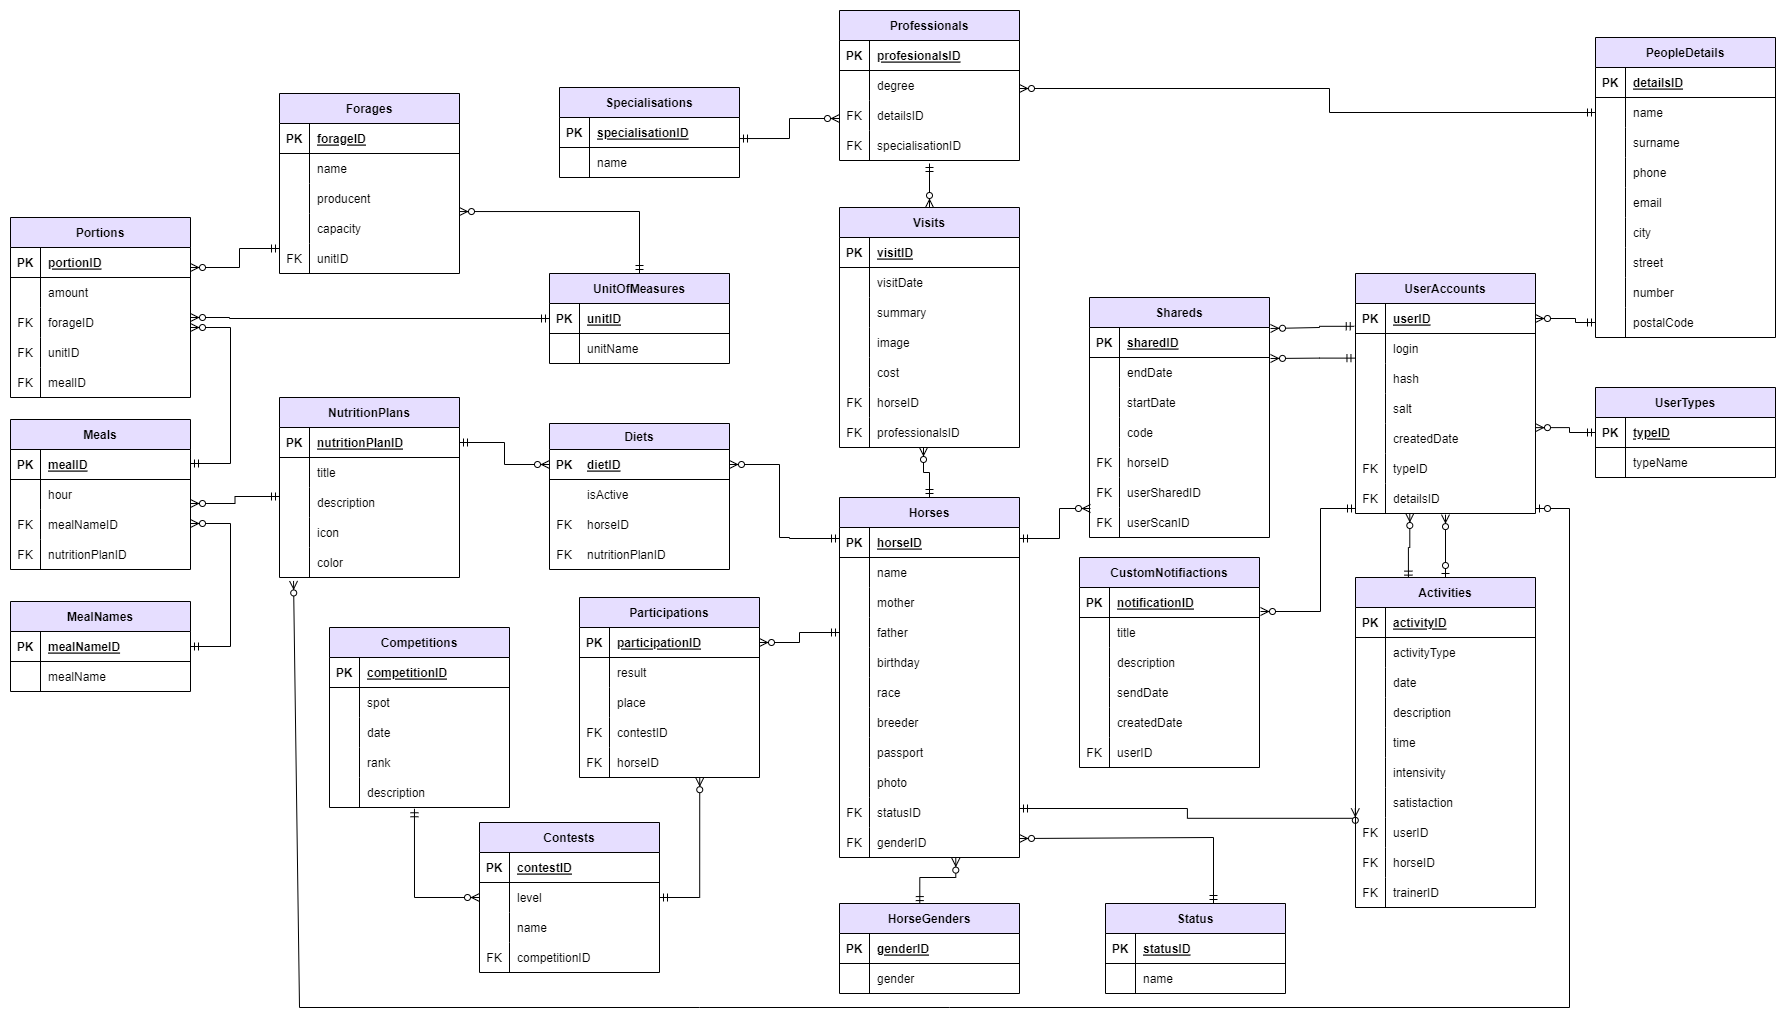
\includegraphics[scale=0.35, angle=-90]{DiagramLogiczny}
	\caption{Logiczny schemat bazy danych}
	\textit{Źródło: Opracowanie własne}
	\label{DiagramLogiczny}
\end{figure}
\newpage
\section{Model fizyczny}
Po stworzeniu logicznego modelu bazy danych, możemy przetransformować go w model fizyczny. Model fizyczny składa się z plików i rekordów. Pilki bazy danych złożony jest z poszczególnych rekordów, przy czym rekordy te mają 
// dokończyć na podstawie książki Sharon Allen
\begin{figure}[H]
	\centering
	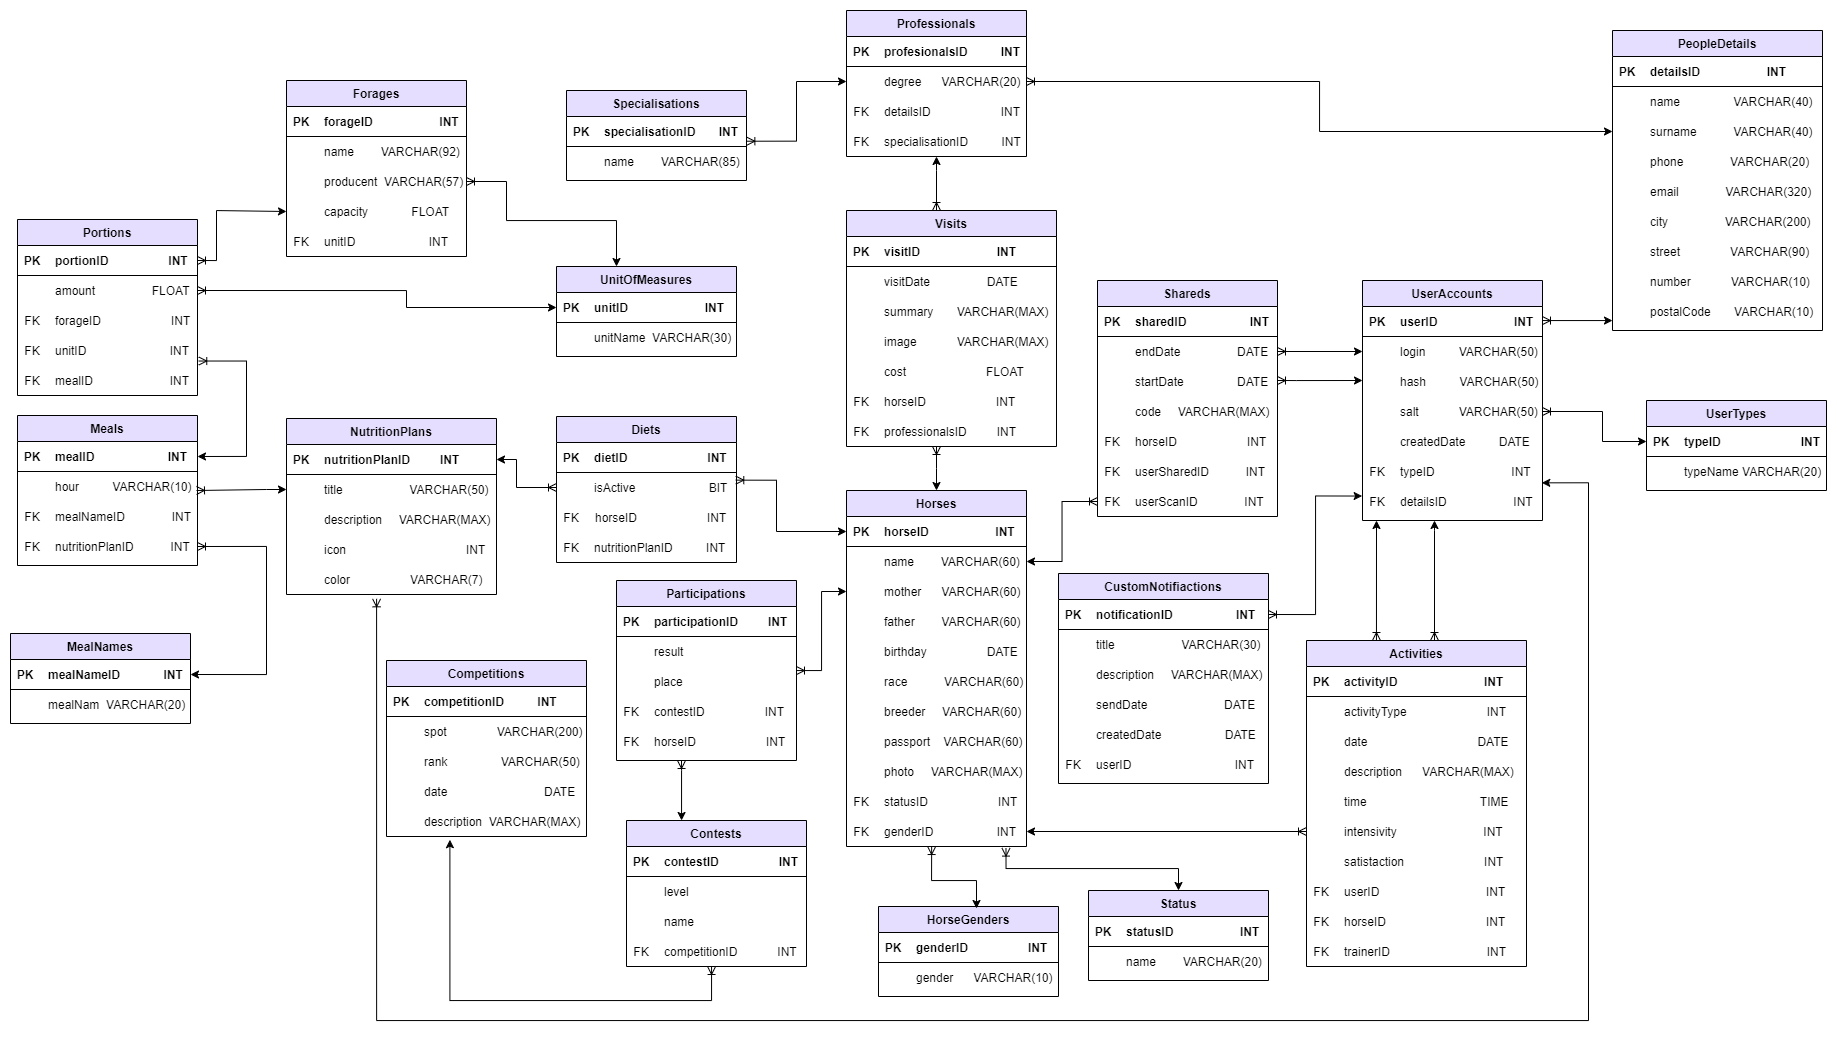
\includegraphics[scale=0.35]{DiagramFizyczny}
	\caption{Fizyczny schemat bazy danych}
	\textit{Źródło: Opracowanie własne}
	\label{DiagramFizyczny}
\end{figure}
\chapter{Projekt systemu}
\section{Model projektowanego systemu}
\subsubsection{Diagramy stanów}
\subsubsection{Diagramy aktywności}
\subsubsection{Diagram klas}
\subsubsection{Architektura aplikacji}
Jaka baza jakie połączenie itp.
\subsubsection{Wykorzystane wzorce projektowe}
\subsubsection{Model architektoniczny MVVM}
\section{Wybrane aspekty implementacyjne}
jeden viewmodel obsługuje dwa widoki (dodawanie aktywności i szczegóły aktywności) \\
kontrolki\\
\chapter{Testy aplikacji}
\section{Unit testy}
\section{Test case}
\section{Baza błędów}
\chapter{Dokumentacja użytkownika}
\section{Aplikacja desktopowa}
\newpage
\section{Aplikacja mobilna}
Aplikacja mobilna "HorseTracking" służy do zapisywania dziennych aktywności koni, ich wizyt u lekarzy, kowali jak także do zarządzania zawodami.

\begin{wrapfigure}{r}{0.5\linewidth}
	\centering
	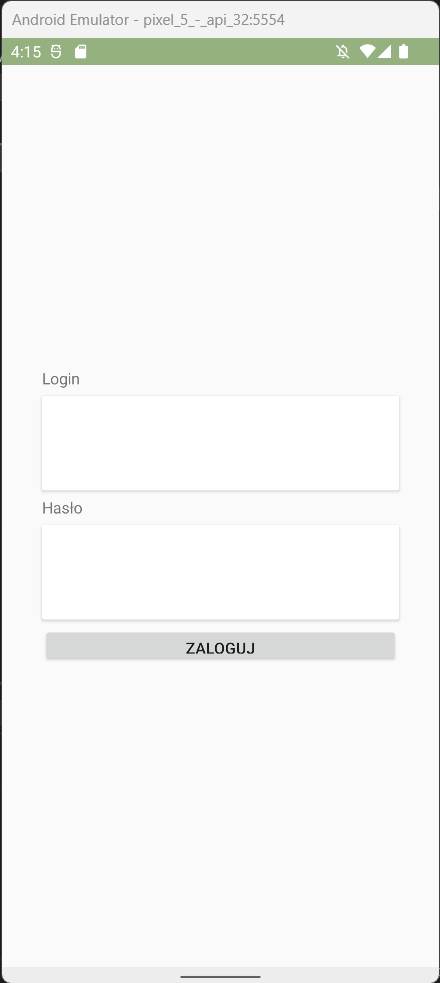
\includegraphics[scale=0.35]{LoginView}
	\caption{\centering Logowanie do aplikacji.}
	\textit{\centering Źródło: Opracowanie własne}
	\label{LoginView}
	\newline
	\newline
		\centering
	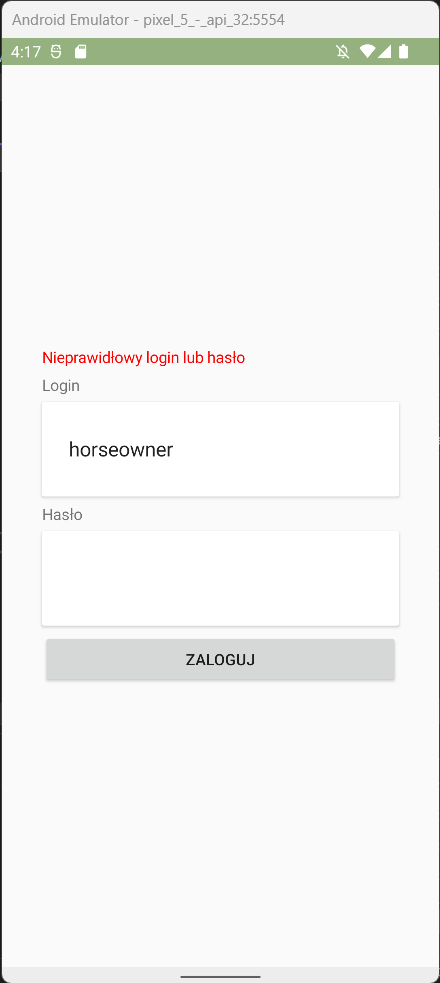
\includegraphics[scale=0.35]{WrongLoginData}
	\caption{\centering Błędne dane logowania.}
	\textit{\centering Źródło: Opracowanie własne}
	\label{LoginViewWrongPassword}
\end{wrapfigure}
Po pierwszym otwarciu aplikacji użytkownikowi ukaże się okno logowania przedstawione na rysunku \ref{LoginView}. 

Na tym ekranie użytkownik może zalogować się do aplikacji. \textcolor{red}{Możliwa jest także opcja zresetowania swojego hasła, w przypadku zapomnienia hasła}. Rejestracja do aplikacji nie jest możliwa, ponieważ ta funkcja jest dostępna jedynie dla administratora w aplikacji desktopowej. Po wprowadzeniu loginu i hasła, a następnie kliknięciu przycisku "Zaloguj" sprawdzana jest poprawność wprowadzonych danych. 

Jeśli przy próbie zalogowania podane zostaną nieprawidłowe dane logowania, bądź użytkownika nie ma w systemie, zostanie on o tym poinformowany (patrz. rys \ref{LoginViewWrongPassword})
Użytkownik nieposiadający koni (użytkownik typu appOwner) nie może zalogować się do aplikacji mobilnej, ponieważ służy ona tylko do wpisywania danych o swoich koniach.

Po poprawnym zalogowaniu się dane użytkownika zostają zapamiętane, więc przy kolejnym otwarciu aplikacji użytkownik będzie już zalogowany.
Aby wylogować się z aplikacji użytkownik musi otworzyć menu boczne i wybrać opcję "Wyloguj".

\begin{wrapfigure}{r}{0.59\textwidth}
	\centering
	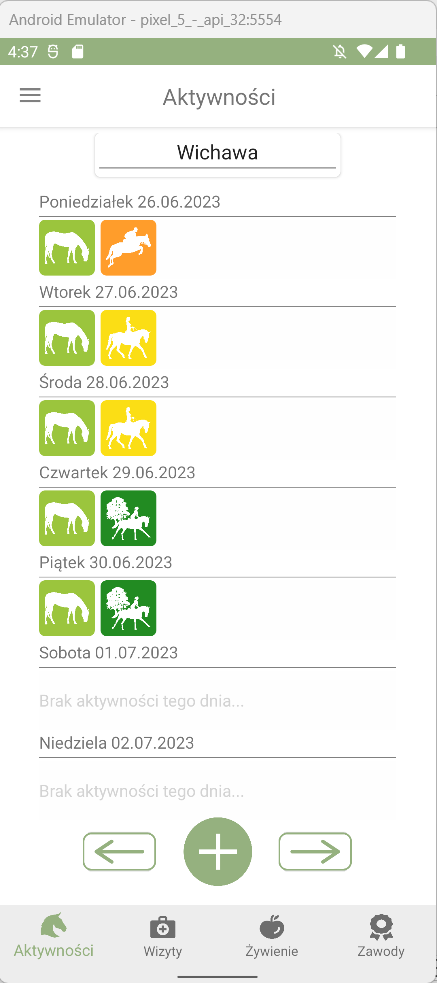
\includegraphics[scale=0.8]{ActivityView}
	\caption{Ekran aktywności.}
	\textit{Źródło: Opracowanie własne}
	\label{ActivityView}
\end{wrapfigure} 

Po zalogowaniu do aplikacji użytkownik zostaje przeniesiony na okno główne. Zawiera ono menu dolne pozwalające na nawigację pomiędzy czterema głównymi sekcjami aplikacji: aktywności, wizyty, żywienie, zawody. Na początek wyświetlona zostaje  strona dotycząca aktywności. W tym widoku można przeglądać informacje o wszystkich aktywnościach koni posiadanych lub tych które trenujemy.  

Aktywności dotyczą konia, którego imię podane jest w polu powyżej. Aby zmienić konia wystarczy kliknąć w to pole i wybrać innego konia.
Strzałki lewo-prawo widoczne na dole ekranu umożliwiają nawigację między kolejnymi tygodniami. W przypadku braku aktywności w danym dniu, wyświetlony jest napis informujący o braku aktywności tego dnia. Każdy typ aktywności ma inny kolor i ikonę, aby ułatwić identyfikacje. Po kliknięciu w daną aktywność możemy przejść do detali dotyczących tej aktywności. Ekran szczegółów został przedstawiony na rysunku \ref{ActivityDetails} i zostanie omówiony później.

Pomiędzy strzałkami nawigującymi miedzy tygodniami znajduje się okrągły przycisk z ikoną "+". Umożliwia on dodawanie aktywności. Dla aktualnie wybranego konia. Przycisk ten dostępny jest jedynie dla właściciela konia oraz osób którym dany koń został udostępniony. Oznacza to, że jeśli użytkownik jest trenerem ta opcja jest dla niego zablokowana, a przycisk nie jest widoczny.

Po kliknięciu w przycisk "+" użytkownik zostaje przeniesiony na okno "Dodawanie aktywności".
\begin{figure}[H]
	\begin{center}
	\begin{minipage}{5cm}
	\centering
	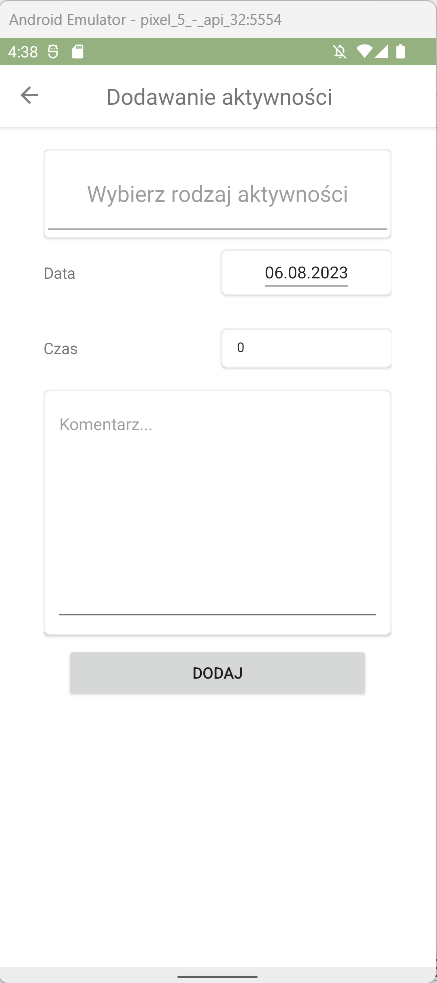
\includegraphics[scale=0.6]{AddActivitySimpleView}
	\caption{\centering Okno dodawania aktywności.}
	\textit{Źródło: Opracowanie własne}
	\label{AddActivitySimple}
\end{minipage}
\hfil
\begin{minipage}{5cm}
	\centering
	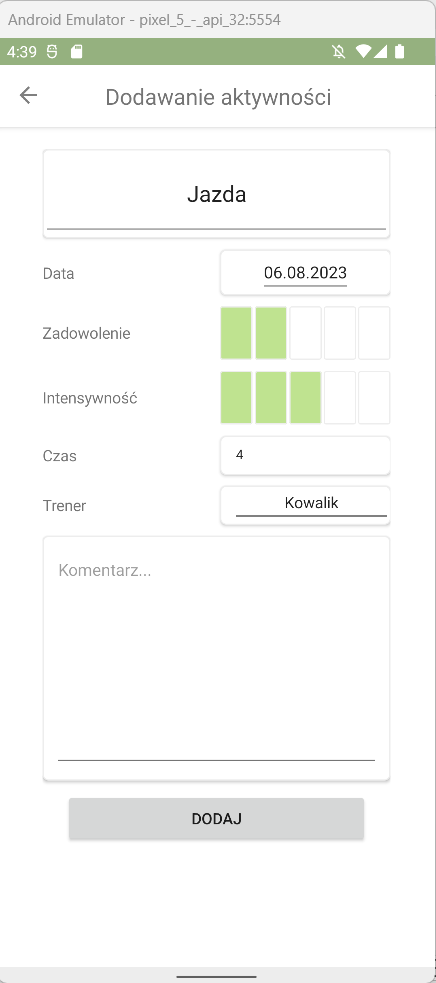
\includegraphics[scale=0.6]{AddActivityAdvancedView}
	\caption{Okno dodawania aktywności rozszerzone.}
	\textit{Źródło: Opracowanie własne}
	\label{AddActivityAdvanced}
\end{minipage}
	\end{center}
\end{figure}
Okno to wygląda różnie w zależności od tego jaki typ aktywności chcemy dodać (patrz rys. \ref{AddActivitySimple} i rys. \ref{AddActivityAdvanced}). Na początku wyświetlony jest prostszy model okna, a po wybraniu typu aktywności dostosowuje się. Dla aktywności: jazda, skoki, zawody, kros czy skoki w oknie dochodzą nowe opcje takie jak satysfakcja, intensywność oraz wybór trenera (patrz. rys \ref{AddActivityAdvanced}). Po uzupełnieniu wszystkich niezbędnych informacji aktywność zostaje dodana i pojawia się na ekranie głównym. Jeśli któraś z niezbędnych informacji nie zostanie uzupełniona aktywność nie doda się, użytkownik zostanie poinformowany o nieprawidłowościach i będzie mógł je poprawić.
\begin{wrapfigure}{r}{0.6\textwidth}
	\centering
	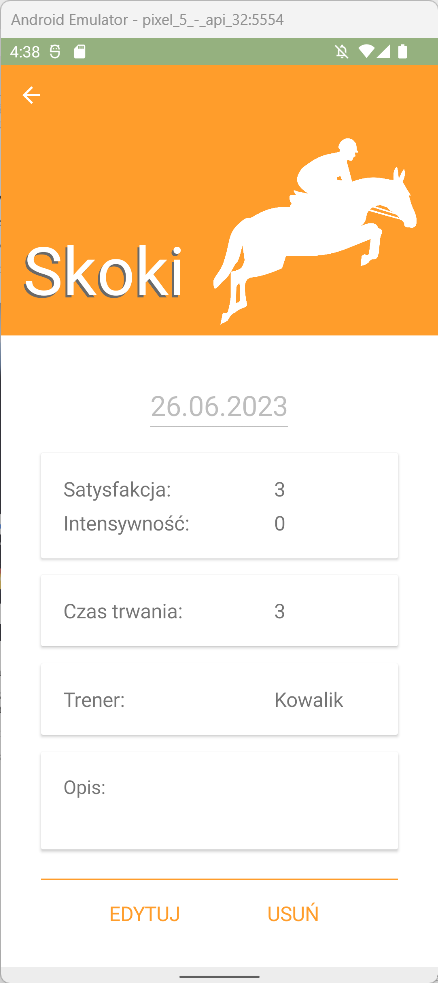
\includegraphics[scale=0.7]{ActivityDetailsView}
	\caption{\centering Szczegóły aktywności.}
	\textit{Źródło: Opracowanie własne}
	\label{ActivityDetails}
\end{wrapfigure}
Po dodaniu aktywności użytkownik zostaje przeniesiony z powrotem na okno główne, gdzie po kliknięciu w wybraną aktywność może zobaczyć jej szczegóły (patrz rys.\ref{ActivityDetails} ). 

W oknie szczegółów oprócz przeczytania wszystkich informacji dotyczących aktywności można także przejść do edycji lub usunąć daną aktywność. Przy edycji otwiera się to samo okno co przy dodawaniu aktywności jednakże tym razem jest ono wypełnione aktualnymi danymi wybranej aktywności. Po zakończonej edycji użytkownik zostaje przeniesiony na okno główne. Po kliknięciu przycisku usuń, wyświetla się komunikat proszący o potwierdzenie wykonania akcji. Jeśli użytkownik potwierdzi, że akcje, to aktywność zostanie usunięta, a użytkownik zostanie przeniesiony na ekran główny. \textcolor{red}{Usunięcie aktywności jest także możliwe poprzez długie przytrzymanie wybranej aktywności na ekranie głównym, a następnie potwierdzenie akcji na pojawiającym się komunikacie.}
\newpage
Kolejną opcją w menu dolnym są wizyty. Na tym oknie podobnie jak w oknie aktywności mamy pole pozwalające wybrać konia o którym informacje chcemy obejrzeć. Koń wybrany na oknie aktywności przenosi się na okno wizyt i na odwrót. W tym oknie można sprawdzić jakie wizyty odbył ostatnio wybrany koń. 
\begin{figure}[H]
	\begin{center}
	\begin{minipage}{5cm}
		\centering
		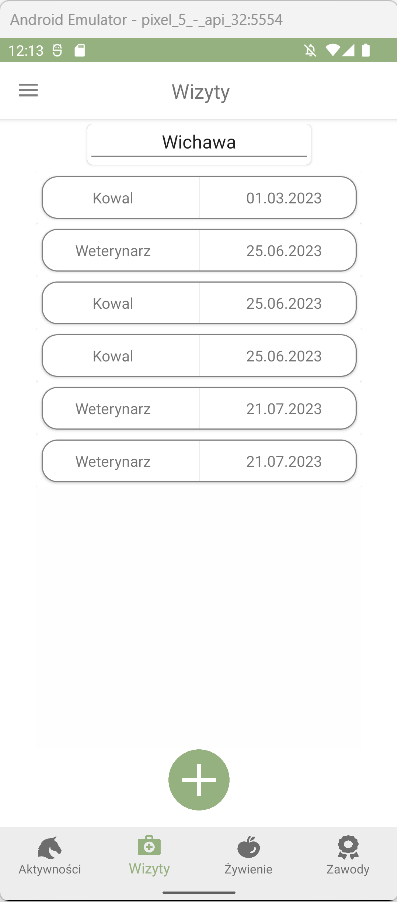
\includegraphics[scale=0.6]{VisitView}
		\caption{\centering Okno wizyt.}
		\textit{Źródło: Opracowanie własne}
		\label{VisitView}
	\end{minipage}
	\hfil
	\begin{minipage}{5cm}
		\centering
		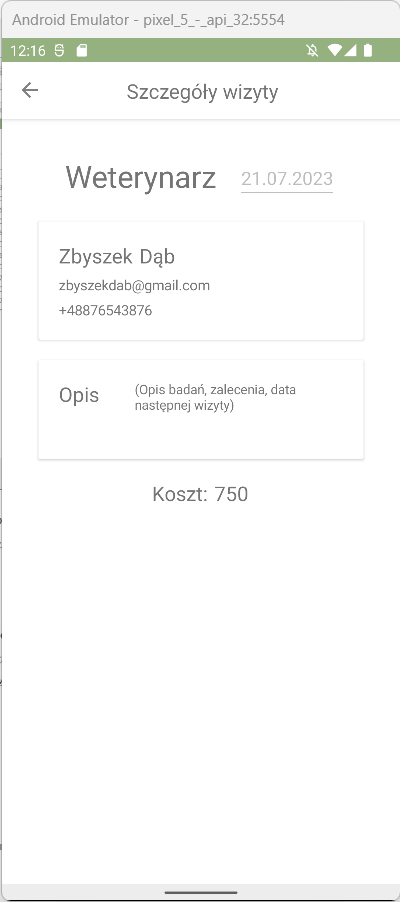
\includegraphics[scale=0.6]{VisitViewDetails}
		\caption{\centering Szczegóły wizyty.}
		\textit{Źródło: Opracowanie własne}
		\label{VisitDetailsView}
	\end{minipage}
\end{center}
\end{figure}
Na rysunku \ref{VisitView} widzimy listę wizyt wybranego konia. Po kliknięciu w wizytę zostaniemy przeniesieni do szczegółów wizyty, gdzie możemy znaleźć dane kontaktowe do lekarza/kowala, który przeprowadził wizytę oraz szczegóły takie jak opis wizyty i jej koszt. Dzięki temu widokowi użytkownik może sprawdzić jakie zalecenia były na poprzednich wizytach, jaki był ich koszt i kiedy dokładnie się odbyły.
\newpage
\begin{wrapfigure}{r}{0.6\textwidth}
	\centering
	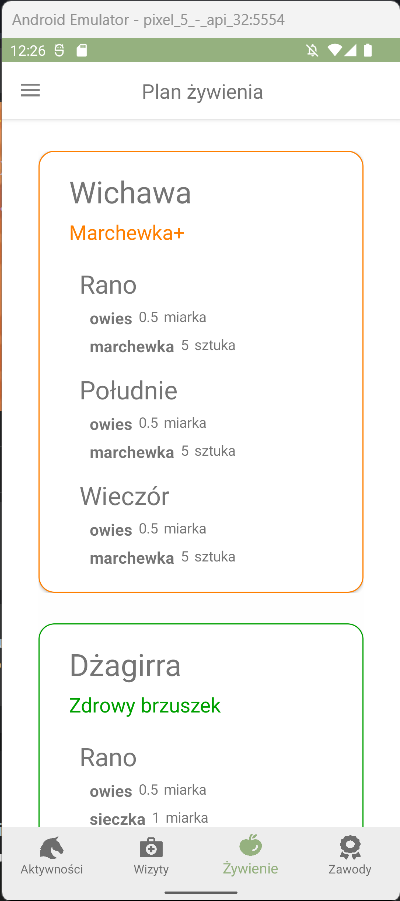
\includegraphics[scale=0.7]{NutritionPlan}
	\caption{\centering Szczegóły aktywności.}
	\textit{Źródło: Opracowanie własne}
	\label{ActivityDetails}
\end{wrapfigure}
Kolejną opcją dostępną w menu dolnym są plany żywienia. Po kliknięciu w ikonę "jabłka" użytkownik zostanie przeniesiony na stronę z planami żywienia wszystkich jego koni. W widoku tym można jedynie obejrzeć plan żywienia, nie jest możliwe ich dodanie, edycja bądź usunięcie. Całość zarządzania planami żywnienia została zaimplementowana w aplikacji desktopowej.

\chapter{Podsumowanie}
\begin{thebibliography}{9}
	
	\bibitem{bazydanych}
	Hanna Mazur, Zygmunt Mazur,
	\emph{Projektowanie relacyjnych baz danych}.
	Oficyna Wydawnicza Politechniki Wrocławskiej, Wrocław 2004.

	\bibitem{XamarinLearn} profexorgeek, alexbuckgit, v-hearya, davidbritch, conceptdev \emph{Co to jest środowisko Xamarin?}
	https://learn.microsoft.com/pl-pl/xamarin/get-started/what-is-xamarin [Dostęp: 06.08.2023] 

	\bibitem{Nuget} JonDouglas, alexbuckgit, Mikejo5000, v-hearya, zivkan, chrisraygill, loic-sharma, karann-msft, NickKruger,	mairaw, kraigb, alfredmyers, \emph{Wprowadzenie do narzędzia NuGet} https://learn.microsoft.com/pl-pl/nuget/what-is-nuget 
	[Dostęp: 06.08.2023]

	\bibitem{Entity}Paweł Łukasiewicz \emph{C\# - Entity Framework} https://www.plukasiewicz.net/Artykuly/EntityFramework
	[Dostęp: 06.08.2023]

	\bibitem{FigmaBlog} Juris Lavrinovics, \emph{Figma - narzędzie do projektowania interfejsu użytkownika}
	https://blog.consdata.tech/2023/02/15/uiux-tools.html 
	[Dostęp 05.05.2023]

	\bibitem{FigmaAbout}https://www.figma.com/about/ 
	[Dostęp 05.05.2023]

	\bibitem{FigmaIcon}Figma \emph{Figma-logo} https://commons.wikimedia.org/wiki/File:Figma-logo.svg 
	[Dostęp 05.05.2023]
	
	\bibitem{WPF} adegeo, ihsansfd, alexbuckgit, v-trisshores, DCtheGeek, \emph{Przewodnik dotyczący aplikacji klasycznych (WPF .NET)}\\ https://learn.microsoft.com/pl-pl/dotnet/desktop/wpf/overview/?view=netdesktop-7.0 
	[Dostęp: 06.08.2023]

\end{thebibliography}
\listoffigures
\lstlistoflistings
\listoftables
\chapter{Opis zawartości APD}


\end{document}